% Options for packages loaded elsewhere
% Options for packages loaded elsewhere
\PassOptionsToPackage{unicode}{hyperref}
\PassOptionsToPackage{hyphens}{url}
\PassOptionsToPackage{dvipsnames,svgnames,x11names}{xcolor}
%
\documentclass[
  letterpaper,
  DIV=11,
  numbers=noendperiod]{scrartcl}
\usepackage{xcolor}
\usepackage{amsmath,amssymb}
\setcounter{secnumdepth}{-\maxdimen} % remove section numbering
\usepackage{iftex}
\ifPDFTeX
  \usepackage[T1]{fontenc}
  \usepackage[utf8]{inputenc}
  \usepackage{textcomp} % provide euro and other symbols
\else % if luatex or xetex
  \usepackage{unicode-math} % this also loads fontspec
  \defaultfontfeatures{Scale=MatchLowercase}
  \defaultfontfeatures[\rmfamily]{Ligatures=TeX,Scale=1}
\fi
\usepackage{lmodern}
\ifPDFTeX\else
  % xetex/luatex font selection
\fi
% Use upquote if available, for straight quotes in verbatim environments
\IfFileExists{upquote.sty}{\usepackage{upquote}}{}
\IfFileExists{microtype.sty}{% use microtype if available
  \usepackage[]{microtype}
  \UseMicrotypeSet[protrusion]{basicmath} % disable protrusion for tt fonts
}{}
\makeatletter
\@ifundefined{KOMAClassName}{% if non-KOMA class
  \IfFileExists{parskip.sty}{%
    \usepackage{parskip}
  }{% else
    \setlength{\parindent}{0pt}
    \setlength{\parskip}{6pt plus 2pt minus 1pt}}
}{% if KOMA class
  \KOMAoptions{parskip=half}}
\makeatother
% Make \paragraph and \subparagraph free-standing
\makeatletter
\ifx\paragraph\undefined\else
  \let\oldparagraph\paragraph
  \renewcommand{\paragraph}{
    \@ifstar
      \xxxParagraphStar
      \xxxParagraphNoStar
  }
  \newcommand{\xxxParagraphStar}[1]{\oldparagraph*{#1}\mbox{}}
  \newcommand{\xxxParagraphNoStar}[1]{\oldparagraph{#1}\mbox{}}
\fi
\ifx\subparagraph\undefined\else
  \let\oldsubparagraph\subparagraph
  \renewcommand{\subparagraph}{
    \@ifstar
      \xxxSubParagraphStar
      \xxxSubParagraphNoStar
  }
  \newcommand{\xxxSubParagraphStar}[1]{\oldsubparagraph*{#1}\mbox{}}
  \newcommand{\xxxSubParagraphNoStar}[1]{\oldsubparagraph{#1}\mbox{}}
\fi
\makeatother


\usepackage{longtable,booktabs,array}
\newcounter{none} % for unnumbered tables
\usepackage{calc} % for calculating minipage widths
% Correct order of tables after \paragraph or \subparagraph
\usepackage{etoolbox}
\makeatletter
\patchcmd\longtable{\par}{\if@noskipsec\mbox{}\fi\par}{}{}
\makeatother
% Allow footnotes in longtable head/foot
\IfFileExists{footnotehyper.sty}{\usepackage{footnotehyper}}{\usepackage{footnote}}
\makesavenoteenv{longtable}
\usepackage{graphicx}
\makeatletter
\newsavebox\pandoc@box
\newcommand*\pandocbounded[1]{% scales image to fit in text height/width
  \sbox\pandoc@box{#1}%
  \Gscale@div\@tempa{\textheight}{\dimexpr\ht\pandoc@box+\dp\pandoc@box\relax}%
  \Gscale@div\@tempb{\linewidth}{\wd\pandoc@box}%
  \ifdim\@tempb\p@<\@tempa\p@\let\@tempa\@tempb\fi% select the smaller of both
  \ifdim\@tempa\p@<\p@\scalebox{\@tempa}{\usebox\pandoc@box}%
  \else\usebox{\pandoc@box}%
  \fi%
}
% Set default figure placement to htbp
\def\fps@figure{htbp}
\makeatother





\setlength{\emergencystretch}{3em} % prevent overfull lines

\providecommand{\tightlist}{%
  \setlength{\itemsep}{0pt}\setlength{\parskip}{0pt}}



 


\KOMAoption{captions}{tableheading}
\makeatletter
\@ifpackageloaded{caption}{}{\usepackage{caption}}
\AtBeginDocument{%
\ifdefined\contentsname
  \renewcommand*\contentsname{Table of contents}
\else
  \newcommand\contentsname{Table of contents}
\fi
\ifdefined\listfigurename
  \renewcommand*\listfigurename{List of Figures}
\else
  \newcommand\listfigurename{List of Figures}
\fi
\ifdefined\listtablename
  \renewcommand*\listtablename{List of Tables}
\else
  \newcommand\listtablename{List of Tables}
\fi
\ifdefined\figurename
  \renewcommand*\figurename{Figure}
\else
  \newcommand\figurename{Figure}
\fi
\ifdefined\tablename
  \renewcommand*\tablename{Table}
\else
  \newcommand\tablename{Table}
\fi
}
\@ifpackageloaded{float}{}{\usepackage{float}}
\floatstyle{ruled}
\@ifundefined{c@chapter}{\newfloat{codelisting}{h}{lop}}{\newfloat{codelisting}{h}{lop}[chapter]}
\floatname{codelisting}{Listing}
\newcommand*\listoflistings{\listof{codelisting}{List of Listings}}
\makeatother
\makeatletter
\makeatother
\makeatletter
\@ifpackageloaded{caption}{}{\usepackage{caption}}
\@ifpackageloaded{subcaption}{}{\usepackage{subcaption}}
\makeatother
\usepackage{bookmark}
\IfFileExists{xurl.sty}{\usepackage{xurl}}{} % add URL line breaks if available
\urlstyle{same}
\hypersetup{
  pdftitle={Trabalho 1 - Demografia},
  pdfauthor={Camila Mesquita, Laíse Ribeiro, Luísa Lopes, Nícolas Baldez - Curitiba (PR)},
  colorlinks=true,
  linkcolor={blue},
  filecolor={Maroon},
  citecolor={Blue},
  urlcolor={Blue},
  pdfcreator={LaTeX via pandoc}}


\title{Trabalho 1 - Demografia}
\author{Camila Mesquita, Laíse Ribeiro, Luísa Lopes, Nícolas Baldez -
Curitiba (PR)}
\date{}
\begin{document}
\maketitle


\subsubsection{\texorpdfstring{\textbf{Questão 1: Diagrama de
Lexis}}{Questão 1: Diagrama de Lexis}}\label{questuxe3o-1-diagrama-de-lexis}

a) Construir o Diagrama de Lexis para os dados de nascidos vivos de 2000
a 2024 da UF escolhida (SINASC) e de óbitos menores de 5 anos (idades
simples) para o mesmo período segundo o ano de nascimento.

\textbf{Resposta:}

\pandocbounded{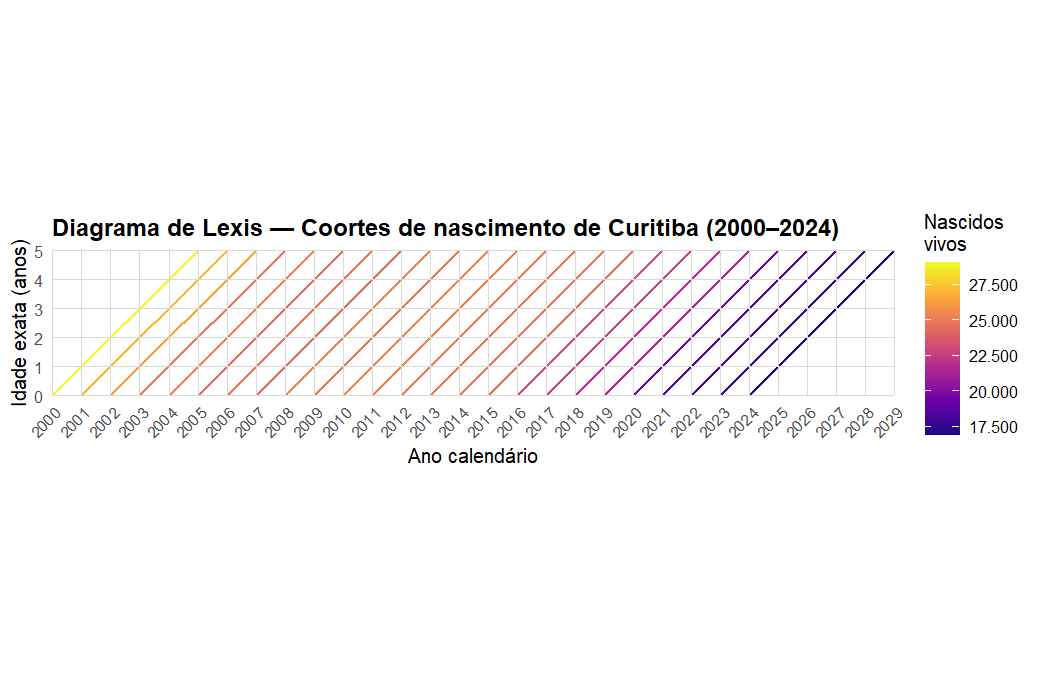
\includegraphics[keepaspectratio]{Rplot03.png}}

\pandocbounded{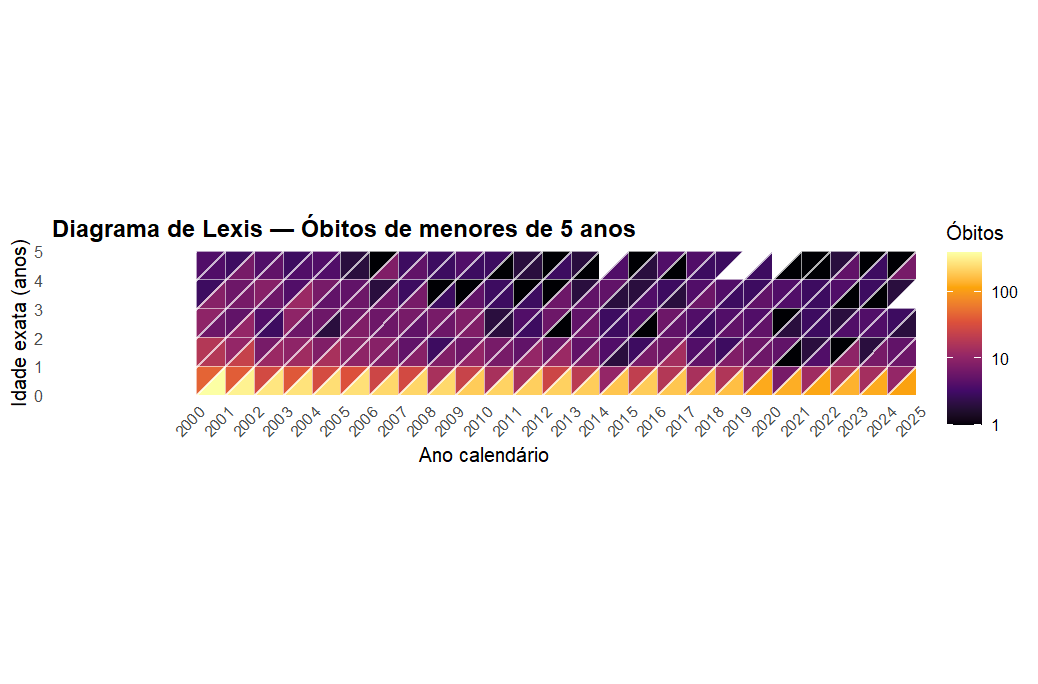
\includegraphics[keepaspectratio]{Rplot04.png}}

b) Supondo população fechada (inexistência de migração), calcule a
probabilidade de um recém-nascido na UF ou no território de escolha
sobreviver à idade exata de 5 para as coortes de 2000 a 2019.

\textbf{Resposta:}

\pandocbounded{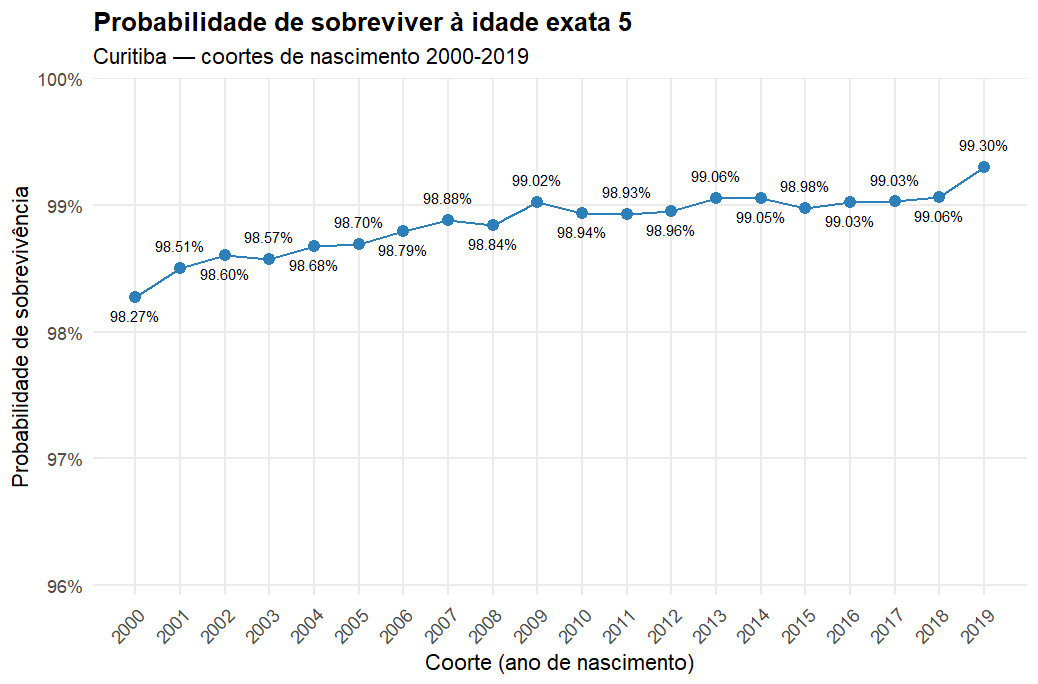
\includegraphics[keepaspectratio]{Rplot06.png}}

c) Considerando o mesmo pressuposto, calcule a probabilidade de
sobreviver ao primeiro aniversário dos recém-nascidos no período de 2000
a 2023.

\textbf{Resposta:}

\pandocbounded{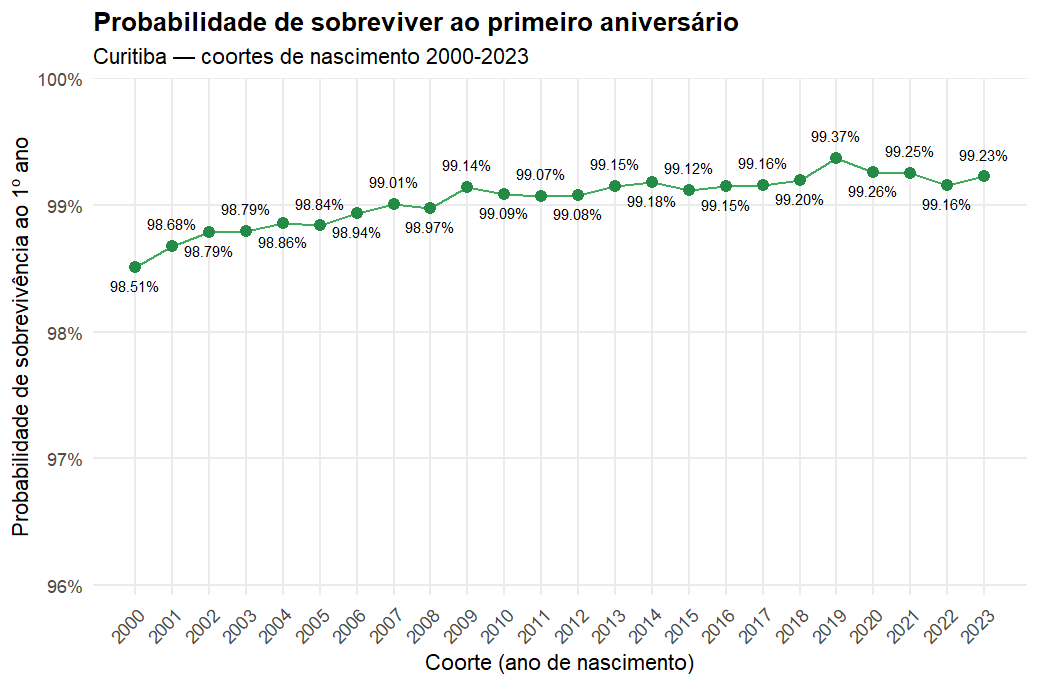
\includegraphics[keepaspectratio]{Rplot07.png}}

d) Para os anos de 2022 e 2023, calcule a probabilidade de morrer antes
de completar o primeiro aniversário, segundo raça/cor (Desafio)

\textbf{Resposta:}

e) Comente os valores encontrados. Não se esquecer da qualidade da
informação trabalhada.

\textbf{Resposta:}

\subsubsection{\texorpdfstring{\textbf{Questão 2:
Natalidade/Fecundidade}}{Questão 2: Natalidade/Fecundidade}}\label{questuxe3o-2-natalidadefecundidade}

a) Com base nos dados do SINASC, para cada um dos anos seguintes: 2010,
2019, 2021, 2022 e 2024, e na população por sexo e idade estimada
(projetada), construa os seguintes indicadores para a Unidade da
Federação (Use as projeções do IBGE - Revisão 2024) :

\begin{itemize}
\item
  Taxa Bruta de Natalidade
\item
  Taxa Fecundidade Geral (TFG) e Taxas específicas de fecundidade - nfx
  (Grafique esses valores)
\item
  Taxa de Fecundidade Total (TFT) ou Índice Sintético de Fecundidade
\item
  Taxas específicas de fecundidade feminina (apenas os nascimentos
  femininos)
\item
  Taxa Bruta de Reprodução
\item
  Taxa Líquida de Reprodução (é necessária a informação da função L da
  Tábua de Vida)
\end{itemize}

\textbf{Resposta:}

\(TBN = \frac{N}{P} \times 1000\)

\(TBN\): Taxa Bruta de Natalidade

\(N\): Número total de nascidos vivos ocorridos no período

\(P\): População média do período

\begin{center}
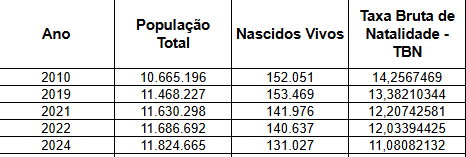
\includegraphics[width=0.7\linewidth,height=\textheight,keepaspectratio]{quest2/TBN.png}
\end{center}

\(TFG = \frac{N}{P_f} \times 1000\)

\(TFG\): Taxa de Fecundidade Geral

\(N\): Número total de nascidos vivos ocorridos no período

\(P_f\): População feminina média entre 15 e 49 anos

\begin{center}
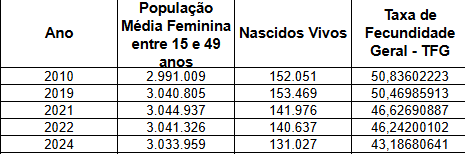
\includegraphics[width=0.7\linewidth,height=\textheight,keepaspectratio]{quest2/TFG.png}
\end{center}

\(nfx = \frac{Nx}{P_fx}\) e \(TEF = \frac{Nx}{Pfx} \times 1000\)

\(nfx\): Nascidos vivos por grupo etário da mãe

\(TEF\): Taxas Específicas de Fecundidade

\(Nx\): Nascidos vivos de mãe entre as idades x e x+n

\(P_fx\): População média feminina entre as idades x e x+n

\begin{center}
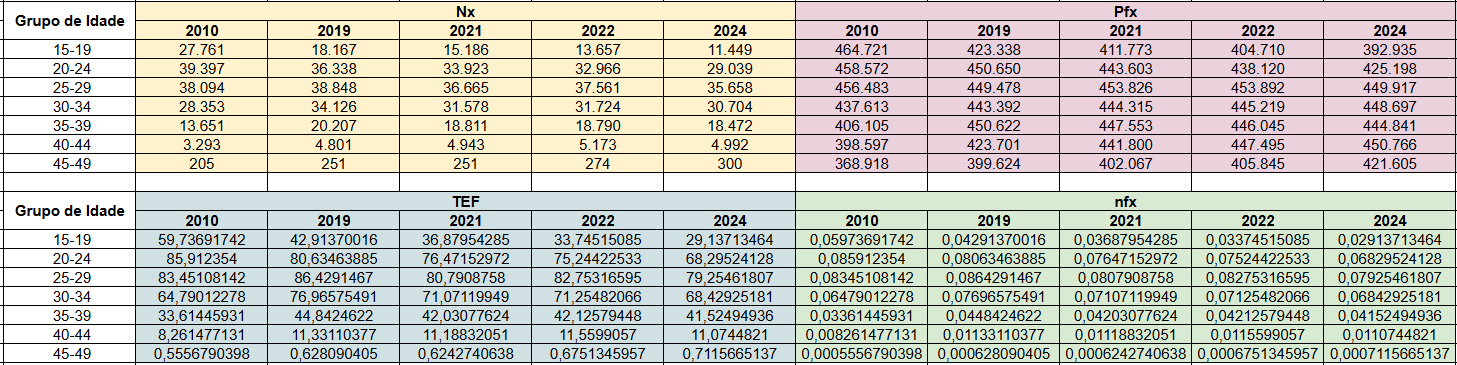
\includegraphics[width=1.1\linewidth,height=\textheight,keepaspectratio]{quest2/TEF_nfx.png}
\end{center}

Gráficos de \(TFG\) e \(nfx\):

\begin{center}
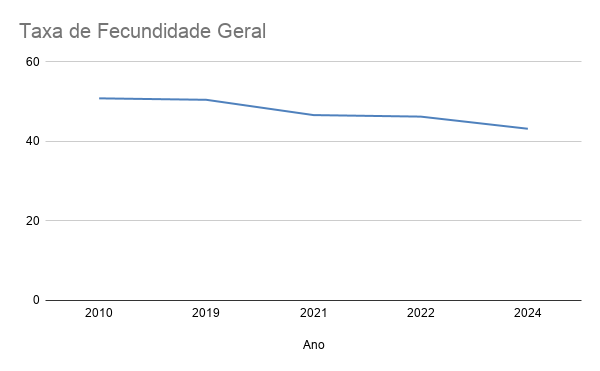
\includegraphics[width=0.7\linewidth,height=\textheight,keepaspectratio]{quest2/TFG_grafico.png}
\end{center}

\begin{center}
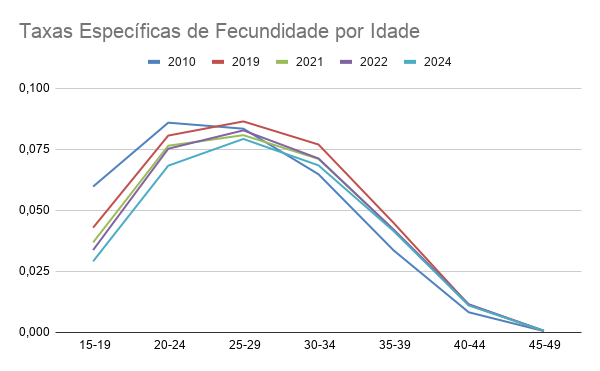
\includegraphics[width=0.7\linewidth,height=\textheight,keepaspectratio]{quest2/nfx_grafico.png}
\end{center}

\(TFT = 5\sum_{i=1}^{7} f_i\)

\(TFT\): Taxa de Fecundidade Total

\(f_i\): grupos quinquenais de \(nfx\)

\begin{center}
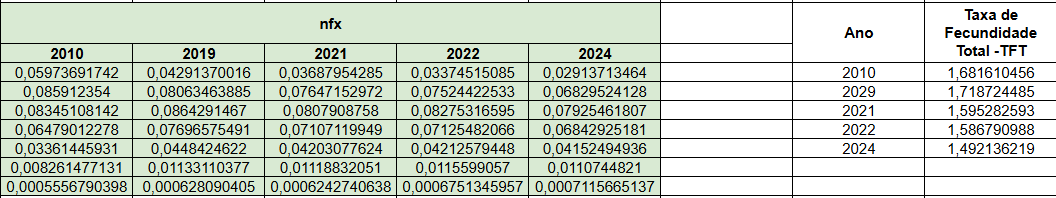
\includegraphics[width=1.1\linewidth,height=\textheight,keepaspectratio]{quest2/TFT.png}
\end{center}

\(f^f_x = \frac{N_f}{P_fx} \times 1000\)

\(f^f_x\): Taxas Específicas de Fecundidade feminina

\(N_f\): Nascidos vivos femininos de mães entre as idades x e x+n

\(P_fx\): População média feminina entre as idades x e x+n

\begin{center}
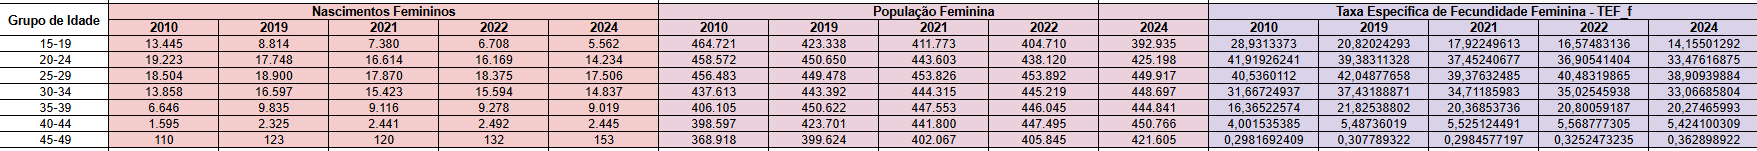
\includegraphics[width=1.1\linewidth,height=\textheight,keepaspectratio]{quest2/TEF_f.png}
\end{center}

\(TBR = 5\sum_{i=1}^{7} f^f_i\)

\(TBR\): Taxa Bruta de Reprodução

\(f^f_i\): grupos quinquenais de \(f^f_x\)

\begin{center}
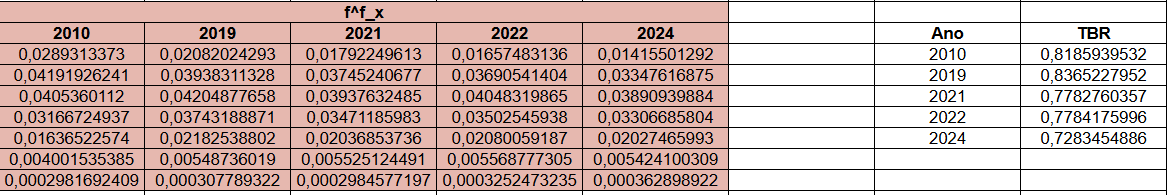
\includegraphics[width=1.1\linewidth,height=\textheight,keepaspectratio]{quest2/TBR.png}
\end{center}

\(TLR = \sum_{i=1}^{7} f^f_i \times\frac{L^f_i}{l_0}\)

\(TLR\): Taxa Líquida de Reprodução

\(f^f_i\): grupos quinquenais de \(f^f_x\)

\(L^f_i\): Função da Tábua de vida

\(l_0\): raiz da Tábua de vida, representa o número de nascimentos

\begin{center}
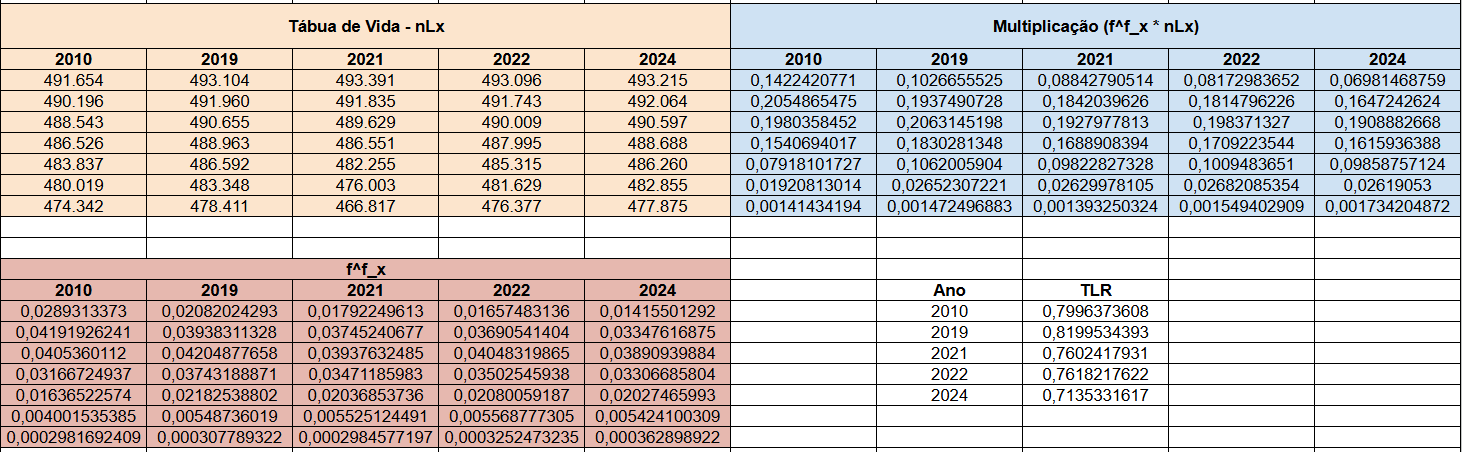
\includegraphics[width=1.1\linewidth,height=\textheight,keepaspectratio]{quest2/TLR.png}
\end{center}

b) Obtenha todos os indicadores de 2022, considerando a população
recenseada nesse ano.

\textbf{Resposta:}

\(TBN\):

\begin{center}
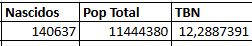
\includegraphics[width=0.4\linewidth,height=\textheight,keepaspectratio]{quest2/TBN2022.png}
\end{center}

\(TFG\):

\begin{center}
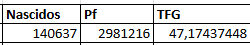
\includegraphics[width=0.4\linewidth,height=\textheight,keepaspectratio]{quest2/TFG2022.png}
\end{center}

\(nfx\) e \(TEF\):

\begin{center}
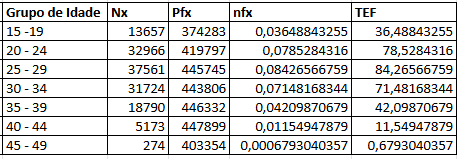
\includegraphics[width=0.4\linewidth,height=\textheight,keepaspectratio]{quest2/TEF_nfx2022.png}
\end{center}

Gráficos de \(TFG\) e \(nfx\):

\begin{center}
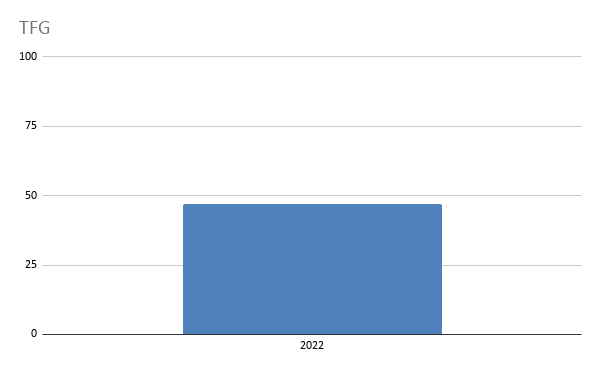
\includegraphics[width=0.4\linewidth,height=\textheight,keepaspectratio]{quest2/TFG_grafico2022.png}
\end{center}

\begin{center}
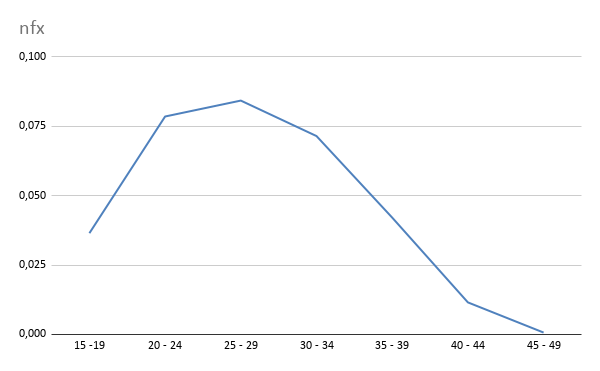
\includegraphics[width=0.4\linewidth,height=\textheight,keepaspectratio]{quest2/nfx_grafico2022.png}
\end{center}

\(TFT\):

\begin{center}
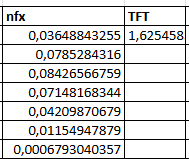
\includegraphics[width=0.35\linewidth,height=\textheight,keepaspectratio]{quest2/TFT2022.png}
\end{center}

\(f^f_x\):

\begin{center}
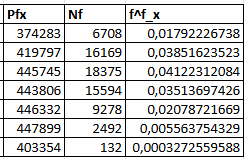
\includegraphics[width=0.4\linewidth,height=\textheight,keepaspectratio]{quest2/ffx2022.png}
\end{center}

\(TBR\):

\begin{center}
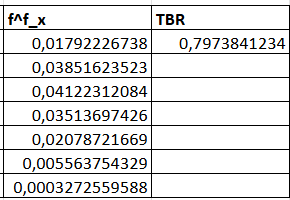
\includegraphics[width=0.4\linewidth,height=\textheight,keepaspectratio]{quest2/TBR2022.png}
\end{center}

\(TLR\):

\begin{center}
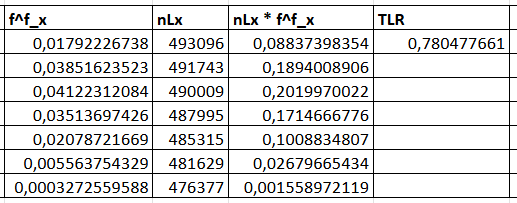
\includegraphics[width=0.7\linewidth,height=\textheight,keepaspectratio]{quest2/TLR2022.png}
\end{center}

c) Comente esses resultados (inclusive os gráficos das nfx), fazendo
referência a artigos já publicados sobre o assunto.

\textbf{Resposta:} As taxas específicas de fecundidade (nfx) aumentam
gradualmente até o grupo de 20 a 29 anos e depois caem bruscamente a
partir do ponto máximo de cada curva. Esse padrão se mantém em todos os
anos analisados (2010, 2019, 2021, 2022 e 2024 - no caso da questão 2a),
indicando que a fecundidade está concentrada nas idades adultas mais
jovens, com poucos nascimentos no início e no final da vida reprodutiva.
As demais taxas apresentam a mesma queda que a nfx. As taxas líquidas de
reprodução, tanto na 2a quanto na 2b, estão abaixo de 1, ou seja, abaixo
do nível de reposição, o que indica que ao longo do tempo, a população
decresce.

d) Para os dados do SINASC para 2024, analise a associação entre
(apresente ao menos uma medida de associação):

\begin{itemize}
\item
  idade (em grupos de idade) e escolaridade da mãe (apresente a tabela
  de contingência e as frequências relativas)
\item
  tipo de parto e escolaridade da mãe (apresente a tabela de
  contingência e as frequências relativas)
\end{itemize}

Apresente graficamente os dados, obtenha medidas para essa associação e
comente os resultados.

\textbf{Resposta:}

Tabela e Gráfico de Contingência Escolaridade por Idade da mãe

\begin{center}
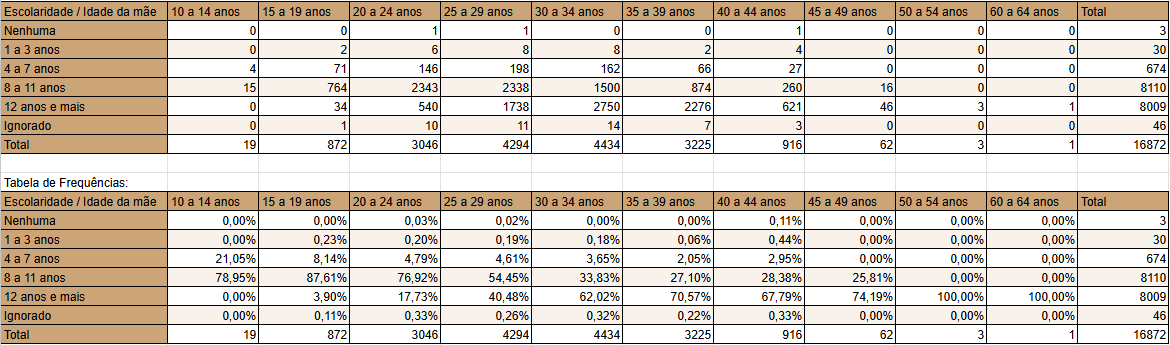
\includegraphics[width=0.7\linewidth,height=\textheight,keepaspectratio]{quest2/TCTF1.png}
\end{center}

\begin{center}
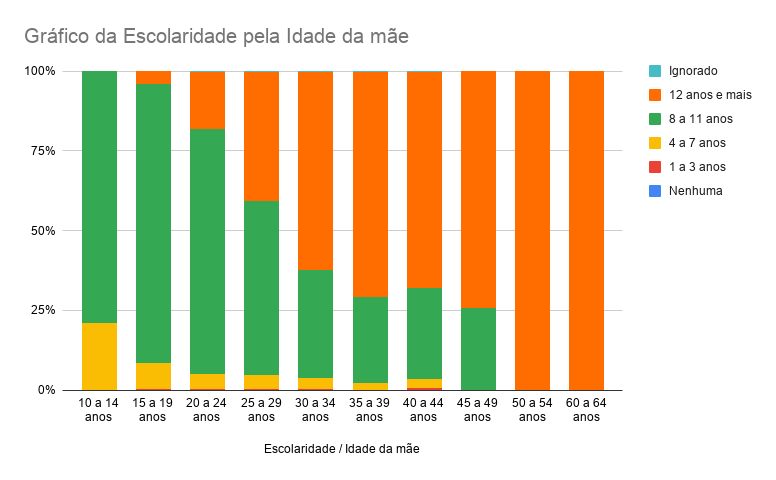
\includegraphics[width=0.7\linewidth,height=\textheight,keepaspectratio]{quest2/grafico1.png}
\end{center}

V de Cramer Interpretação \textless{} 0,10 Associação muito fraca 0,10 -
0,30 Associação fraca 0,30 - 0,50 Associação moderada 0,50 Associação
forte Resumo para sua resposta: Análise Medida Valor Interpretação Idade
vs.~Escolaridade V de Cramer = 0,155 Entre 0,10-0,30 Associação fraca
Parto vs.~Escolaridade RP = 1,67 1 Escolaridade alta é fator de risco
para cesárea (67\% mais chance) Parto vs.~Escolaridade RP = 0,60
\textless{} 1 Escolaridade alta é fator de proteção contra cesárea (40\%
menos chance)

Análise (v de cramer = 0.1932063)

Tabela e Gráfico da Escolaridade pelo Tipo de parto da mãe

\begin{center}
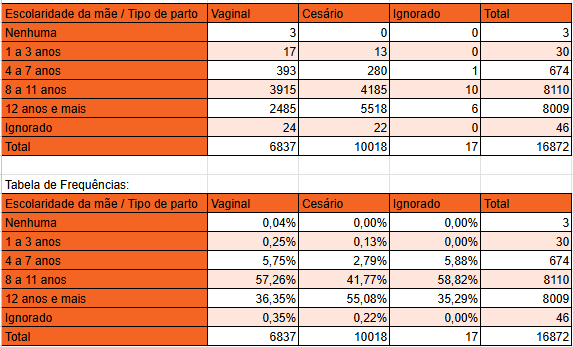
\includegraphics[width=0.7\linewidth,height=\textheight,keepaspectratio]{quest2/TCTF2.png}
\end{center}

\begin{center}
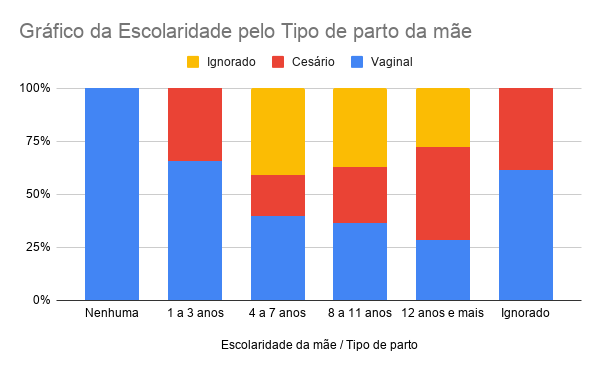
\includegraphics[width=0.7\linewidth,height=\textheight,keepaspectratio]{quest2/grafico2.png}
\end{center}

Análise (v de cramer = 0.1337143/ associação fraca (0.10-0.15))

\subsubsection{\texorpdfstring{\textbf{Questão 3:
Mortalidade}}{Questão 3: Mortalidade}}\label{questuxe3o-3-mortalidade}

a) Com base nos dados sobre óbitos do SIM para os anos: 2010, 2019,
2021, 2022 e 2024 e a população por sexo e idade estimada (projetada)
para a UF ou território escolhido, obtenha os seguintes indicadores:

\begin{itemize}
\item
  Taxa Bruta de Mortalidade
\item
  Taxas específicas de mortalidade por sexo e idade - nMx (grafique)
\end{itemize}

\textbf{Resposta:}

\(Taxa\ Bruta\ de\ Mortalidade\):

\begin{center}
\pandocbounded{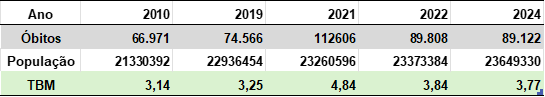
\includegraphics[keepaspectratio]{questao-3/tbm.png}}
\end{center}

\(Taxas\ Específicas\ de\ Mortalidade\ por\ sexo\ e\ idade\)

\begin{itemize}
\tightlist
\item
  2010
\end{itemize}

\begin{center}
\pandocbounded{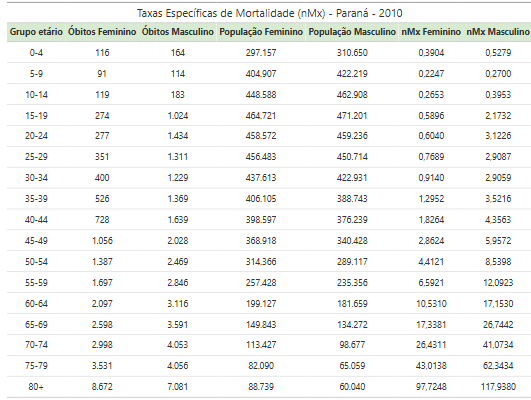
\includegraphics[keepaspectratio]{questao-3/tabela_nmx_2010.png}}
\end{center}

\begin{center}
\pandocbounded{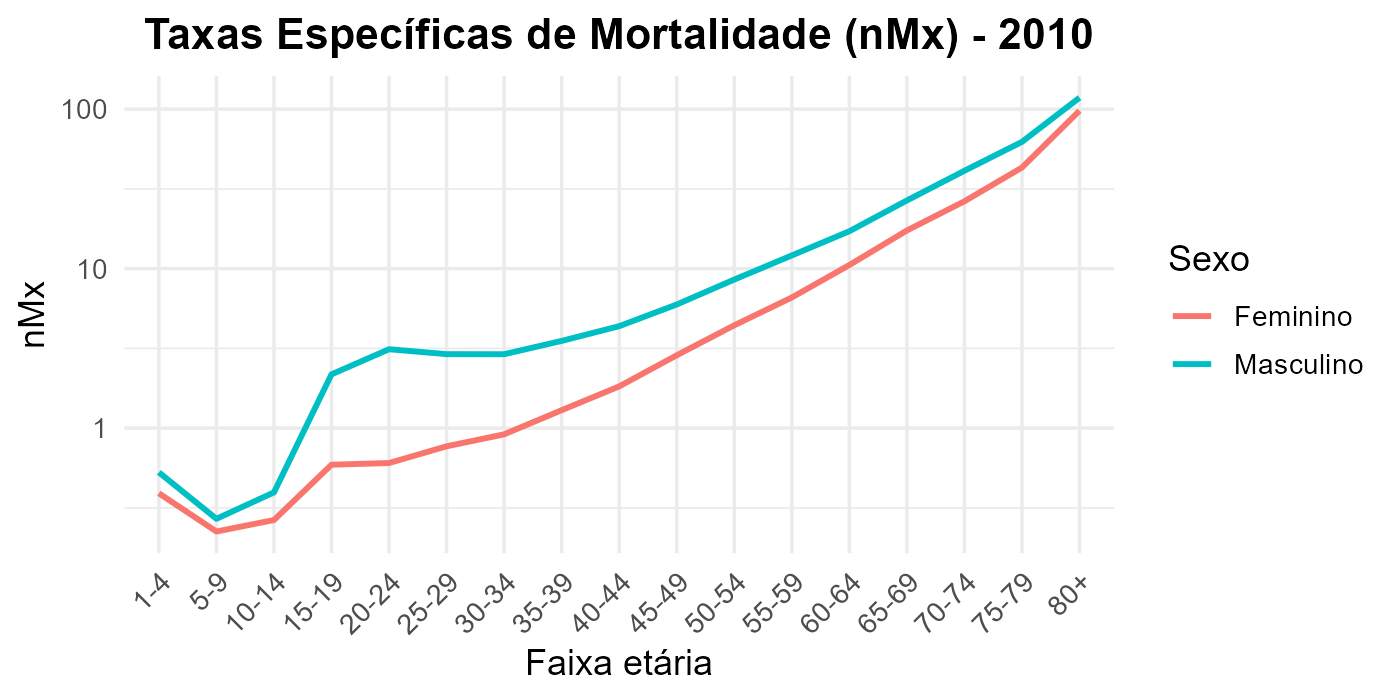
\includegraphics[keepaspectratio]{questao-3/grafico_nmx_2010.png}}
\end{center}

\begin{itemize}
\tightlist
\item
  2019
\end{itemize}

\begin{center}
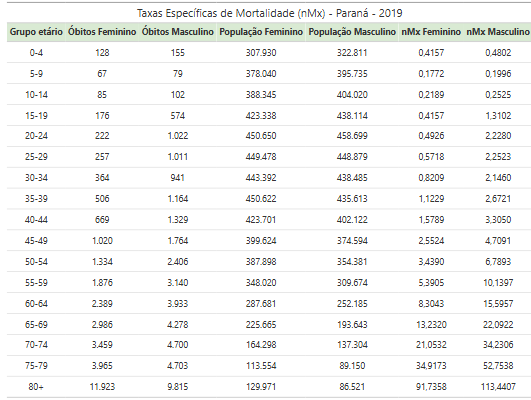
\includegraphics[width=1\linewidth,height=\textheight,keepaspectratio]{questao-3/tabela_nmx_2019.png}
\end{center}

\begin{center}
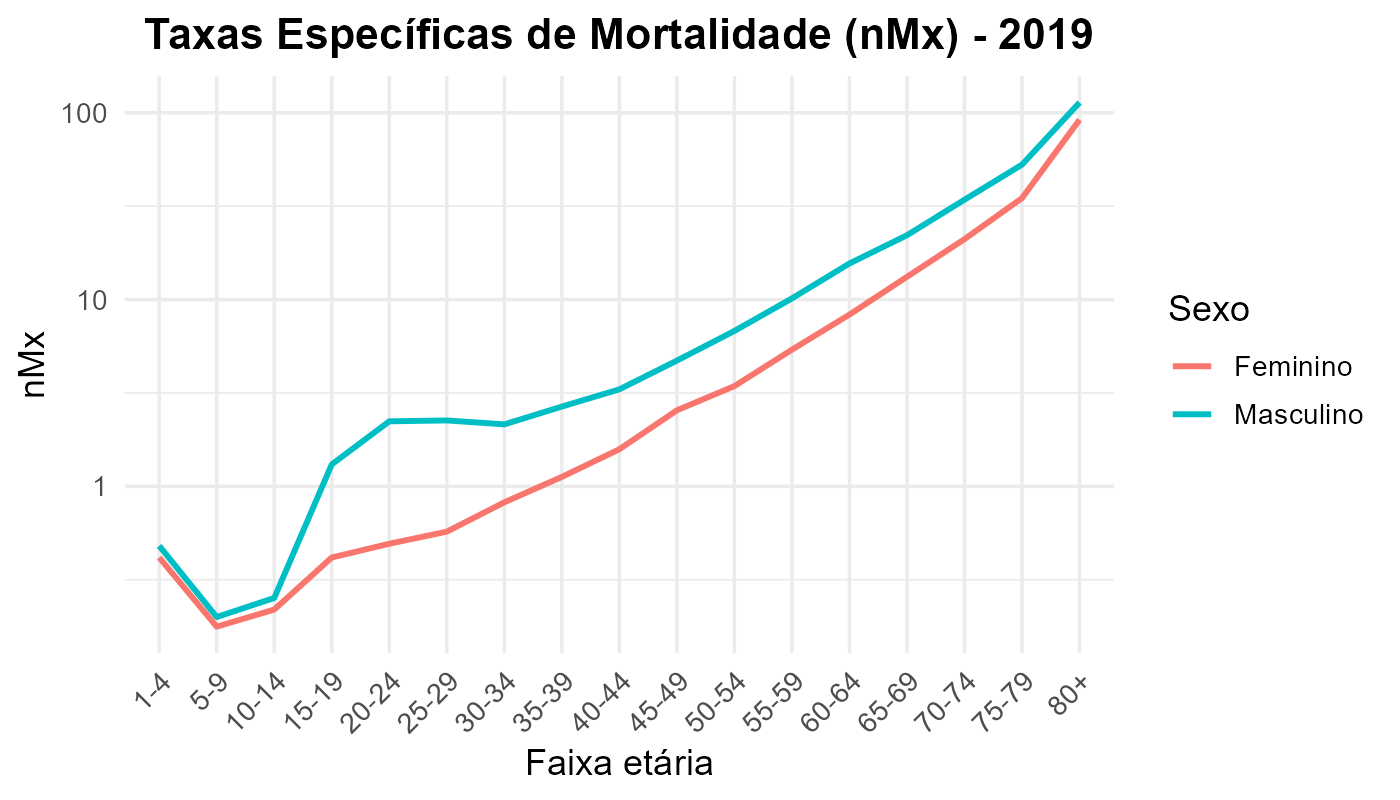
\includegraphics[width=1\linewidth,height=\textheight,keepaspectratio]{questao-3/grafico_nmx_2019.png}
\end{center}

\begin{itemize}
\tightlist
\item
  2021
\end{itemize}

\begin{center}
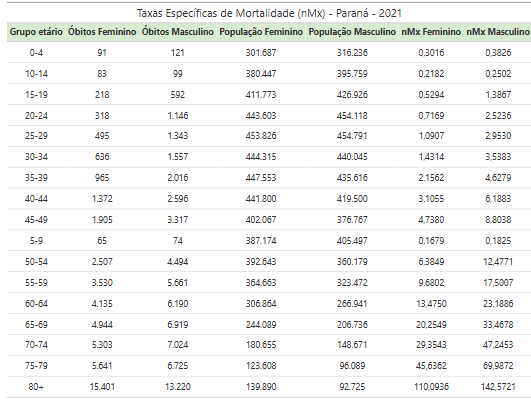
\includegraphics[width=1\linewidth,height=\textheight,keepaspectratio]{questao-3/tabela_nmx_2021.png}
\end{center}

\begin{center}
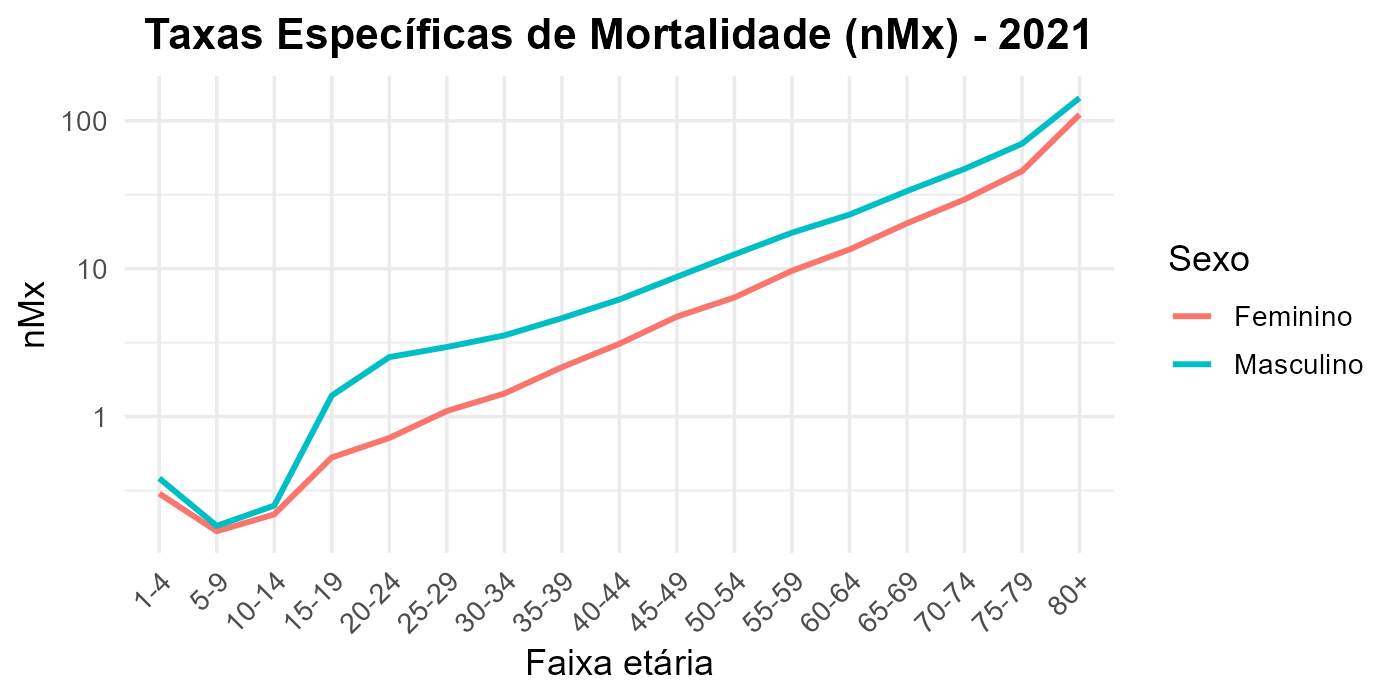
\includegraphics[width=1\linewidth,height=\textheight,keepaspectratio]{questao-3/grafico_nmx_2021.png}
\end{center}

\begin{itemize}
\tightlist
\item
  2022
\end{itemize}

\begin{center}
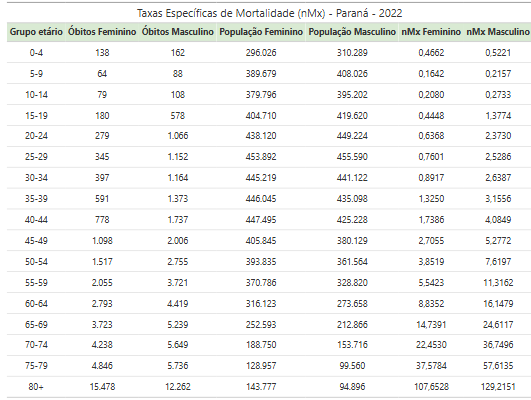
\includegraphics[width=1\linewidth,height=\textheight,keepaspectratio]{questao-3/tabela_nmx_2022.png}
\end{center}

\begin{center}
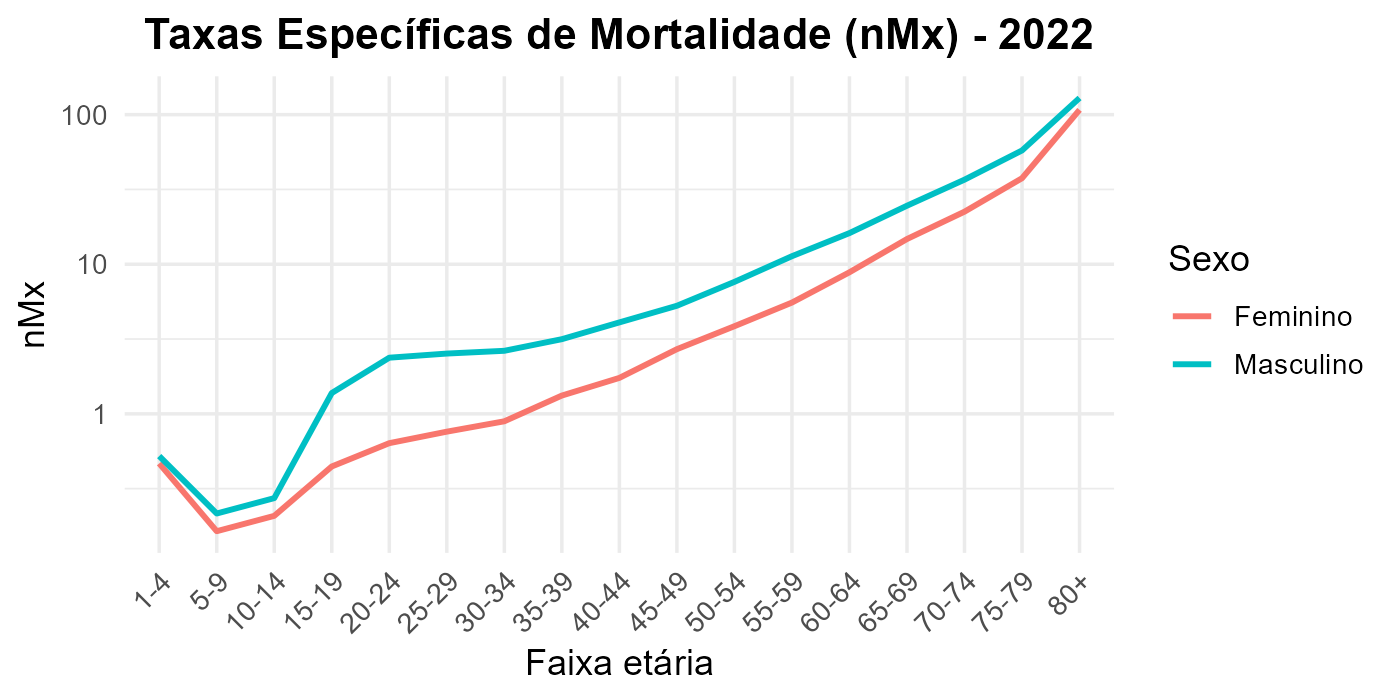
\includegraphics[width=1\linewidth,height=\textheight,keepaspectratio]{questao-3/grafico_nmx_2022.png}
\end{center}

\begin{itemize}
\tightlist
\item
  2024
\end{itemize}

\begin{center}
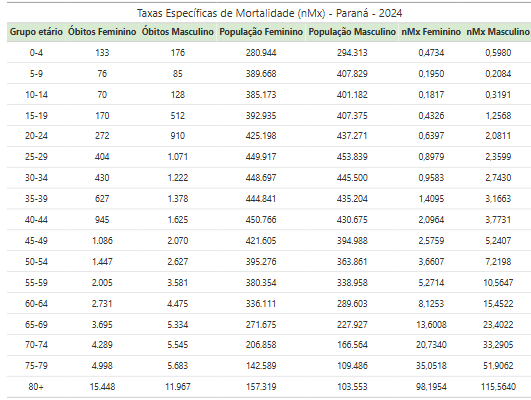
\includegraphics[width=1\linewidth,height=\textheight,keepaspectratio]{questao-3/tabela_nmx_2024.png}
\end{center}

\begin{center}
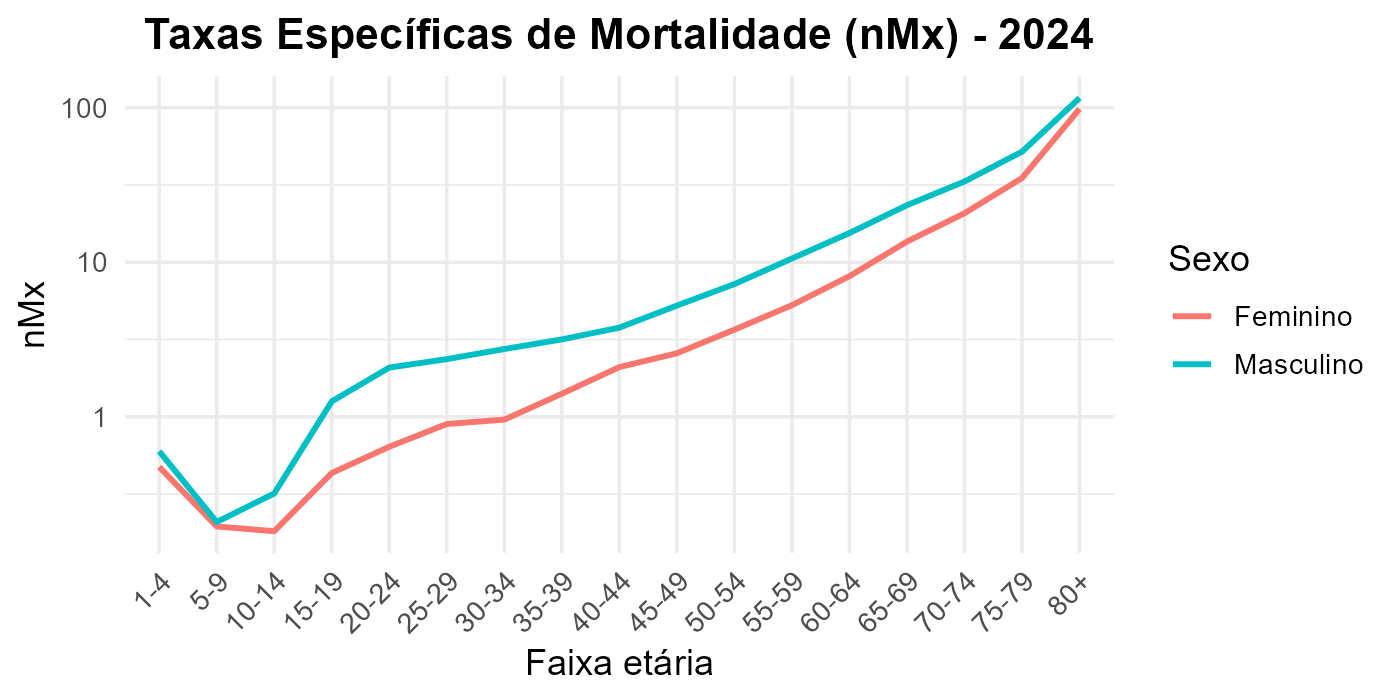
\includegraphics[width=1\linewidth,height=\textheight,keepaspectratio]{questao-3/grafico_nmx_2024.png}
\end{center}

\begin{itemize}
\tightlist
\item
  Comparação anual
\end{itemize}

\begin{center}
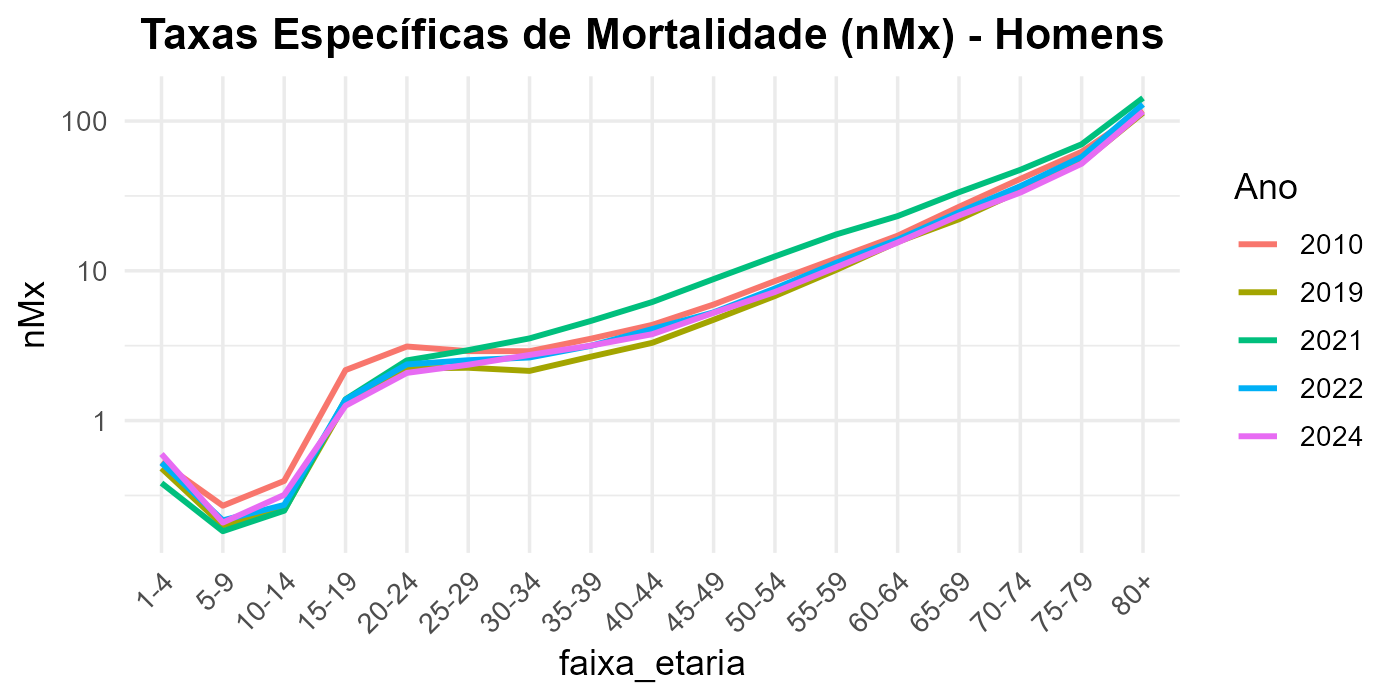
\includegraphics[width=1\linewidth,height=\textheight,keepaspectratio]{questao-3/nmx_homens.png}
\end{center}

\begin{center}
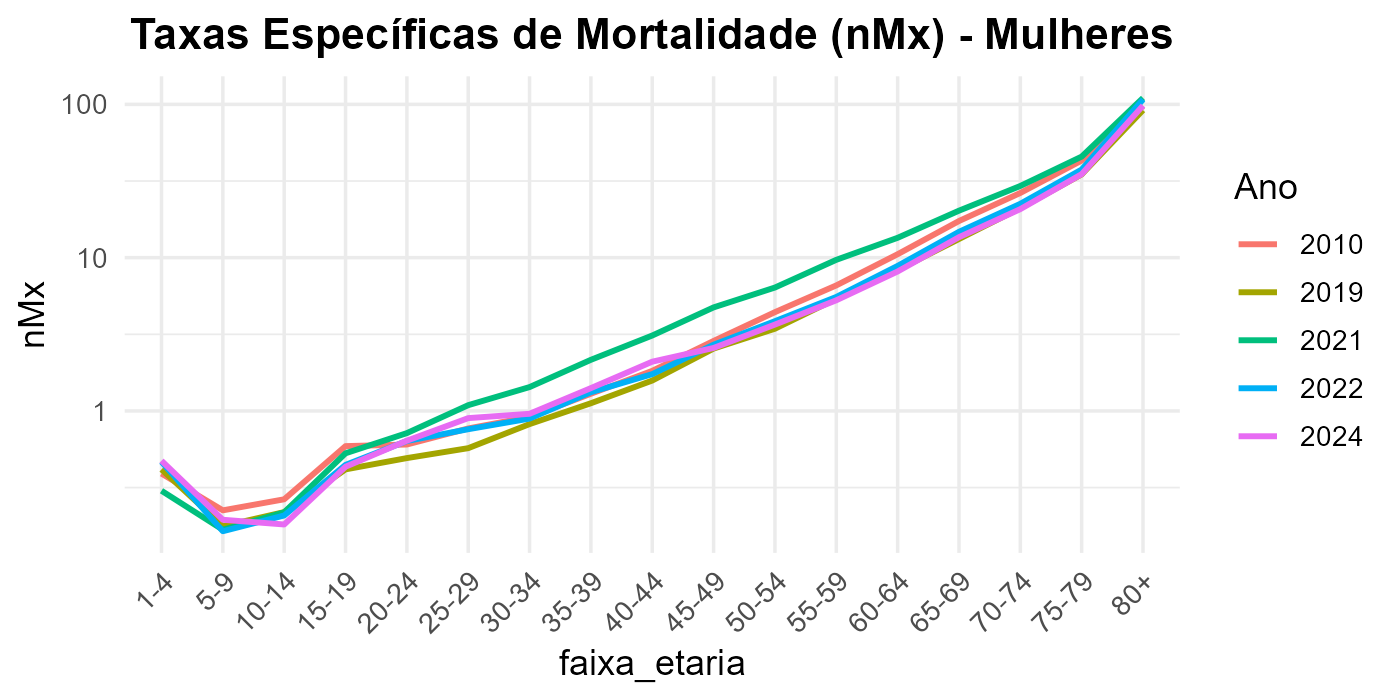
\includegraphics[width=1\linewidth,height=\textheight,keepaspectratio]{questao-3/nmx_mulheres.png}
\end{center}

b) Calcule a TMI, utilizando o \textbf{número médio de óbitos ocorridos
entre 2022 e 2024 (numerador) e o número de nascimentos de 2023
(denominador}). Calcule os indicadores: taxa de mortalidade neonatal,
neonatal precoce, neonatal tardia, posneonatal. A partir da informação
sobre óbitos fetais dos mesmos anos, calcule a taxa de mortalidade
perinatal.

\textbf{Resposta:}

\begin{center}
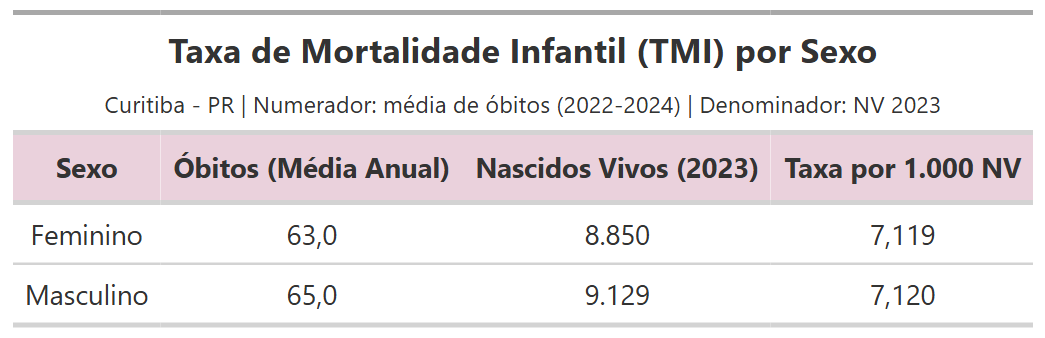
\includegraphics[width=1\linewidth,height=\textheight,keepaspectratio]{questao-3/tabela_4_tmi_por_sexo.png}
\end{center}

\begin{center}
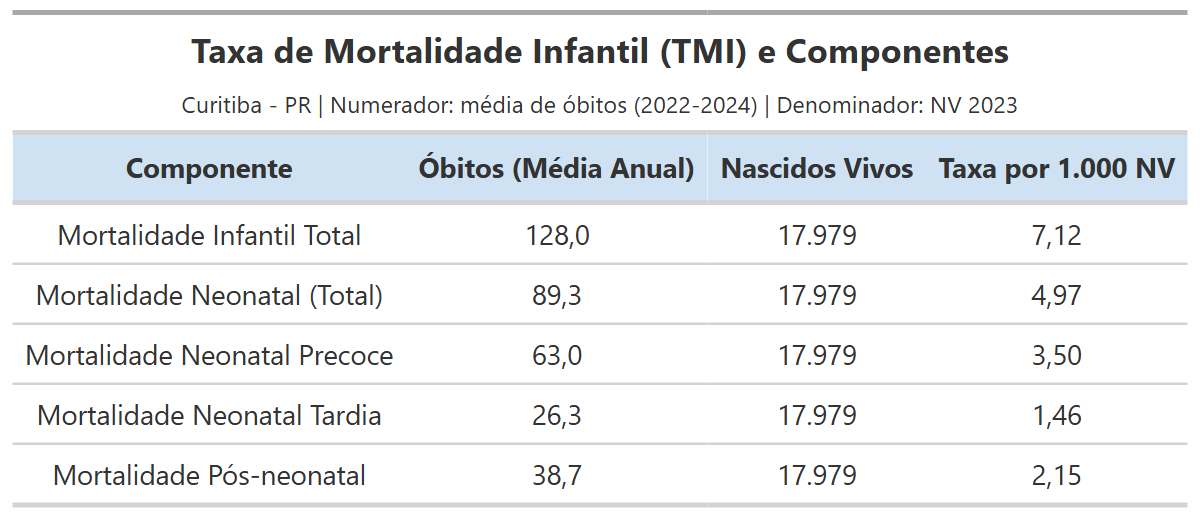
\includegraphics[width=1\linewidth,height=\textheight,keepaspectratio]{questao-3/tabela_1_mortalidade_infantil.png}
\end{center}

\begin{center}
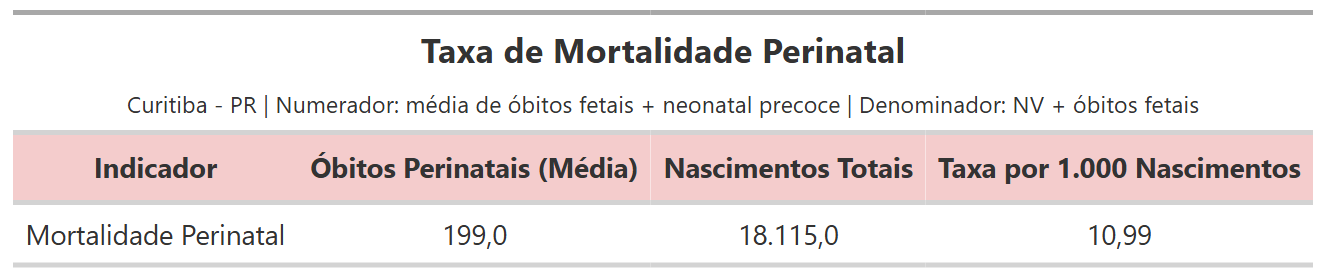
\includegraphics[width=1\linewidth,height=\textheight,keepaspectratio]{questao-3/tabela_2_mortalidade_perinatal.png}
\end{center}

Ao analisar a Taxa de Mortalidade Infantil desagregada por sexo para
Curitiba, observa-se que as taxas para os sexos feminino e masculino
apresentaram-se praticamente idênticas, 7,119 para mulheres e 7,120 para
homens. A literatura demográfica aponta para uma sobremortalidade
masculina na infância, decorrente de fatores biológicos e genéticos. Em
termos absolutos, o volume médio anual de óbitos masculinos no triênio
2022-2024 foi superior ao feminino (65,0 contra 63,0 óbitos). Contudo, a
base de nascidos vivos do sexo masculino em 2023 também foi
proporcionalmente maior (9.129 meninos contra 8.850 meninas), seguindo a
tendência demográfica natural de que nascem mais homens do que mulheres.
Ao efetuar o cálculo da TMI para o sexo feminino e para o sexo
masculino, a maior base de nascimentos masculinos gerou um efeito de
``diluição'' sobre o seu respectivo número de óbitos, resultando em
taxas bem parecidas para ambos os sexos.

c) Compare a estrutura de mortalidade por causas entre 2010, 2021 e
2024. Utilize 20 grupos de causas mais frequentes, segundo os grupos do
CID-10 (ver Tabnet - Datasus), por sexo, e grupos de idade (\textless5;
5 a 14; 15-39; 40-59; 60 e +) para os anos selecionados. Comente os
resultados. Destacar a mortalidade por Covid-19 (CID B34.2).

\textbf{Resposta:}

\begin{center}
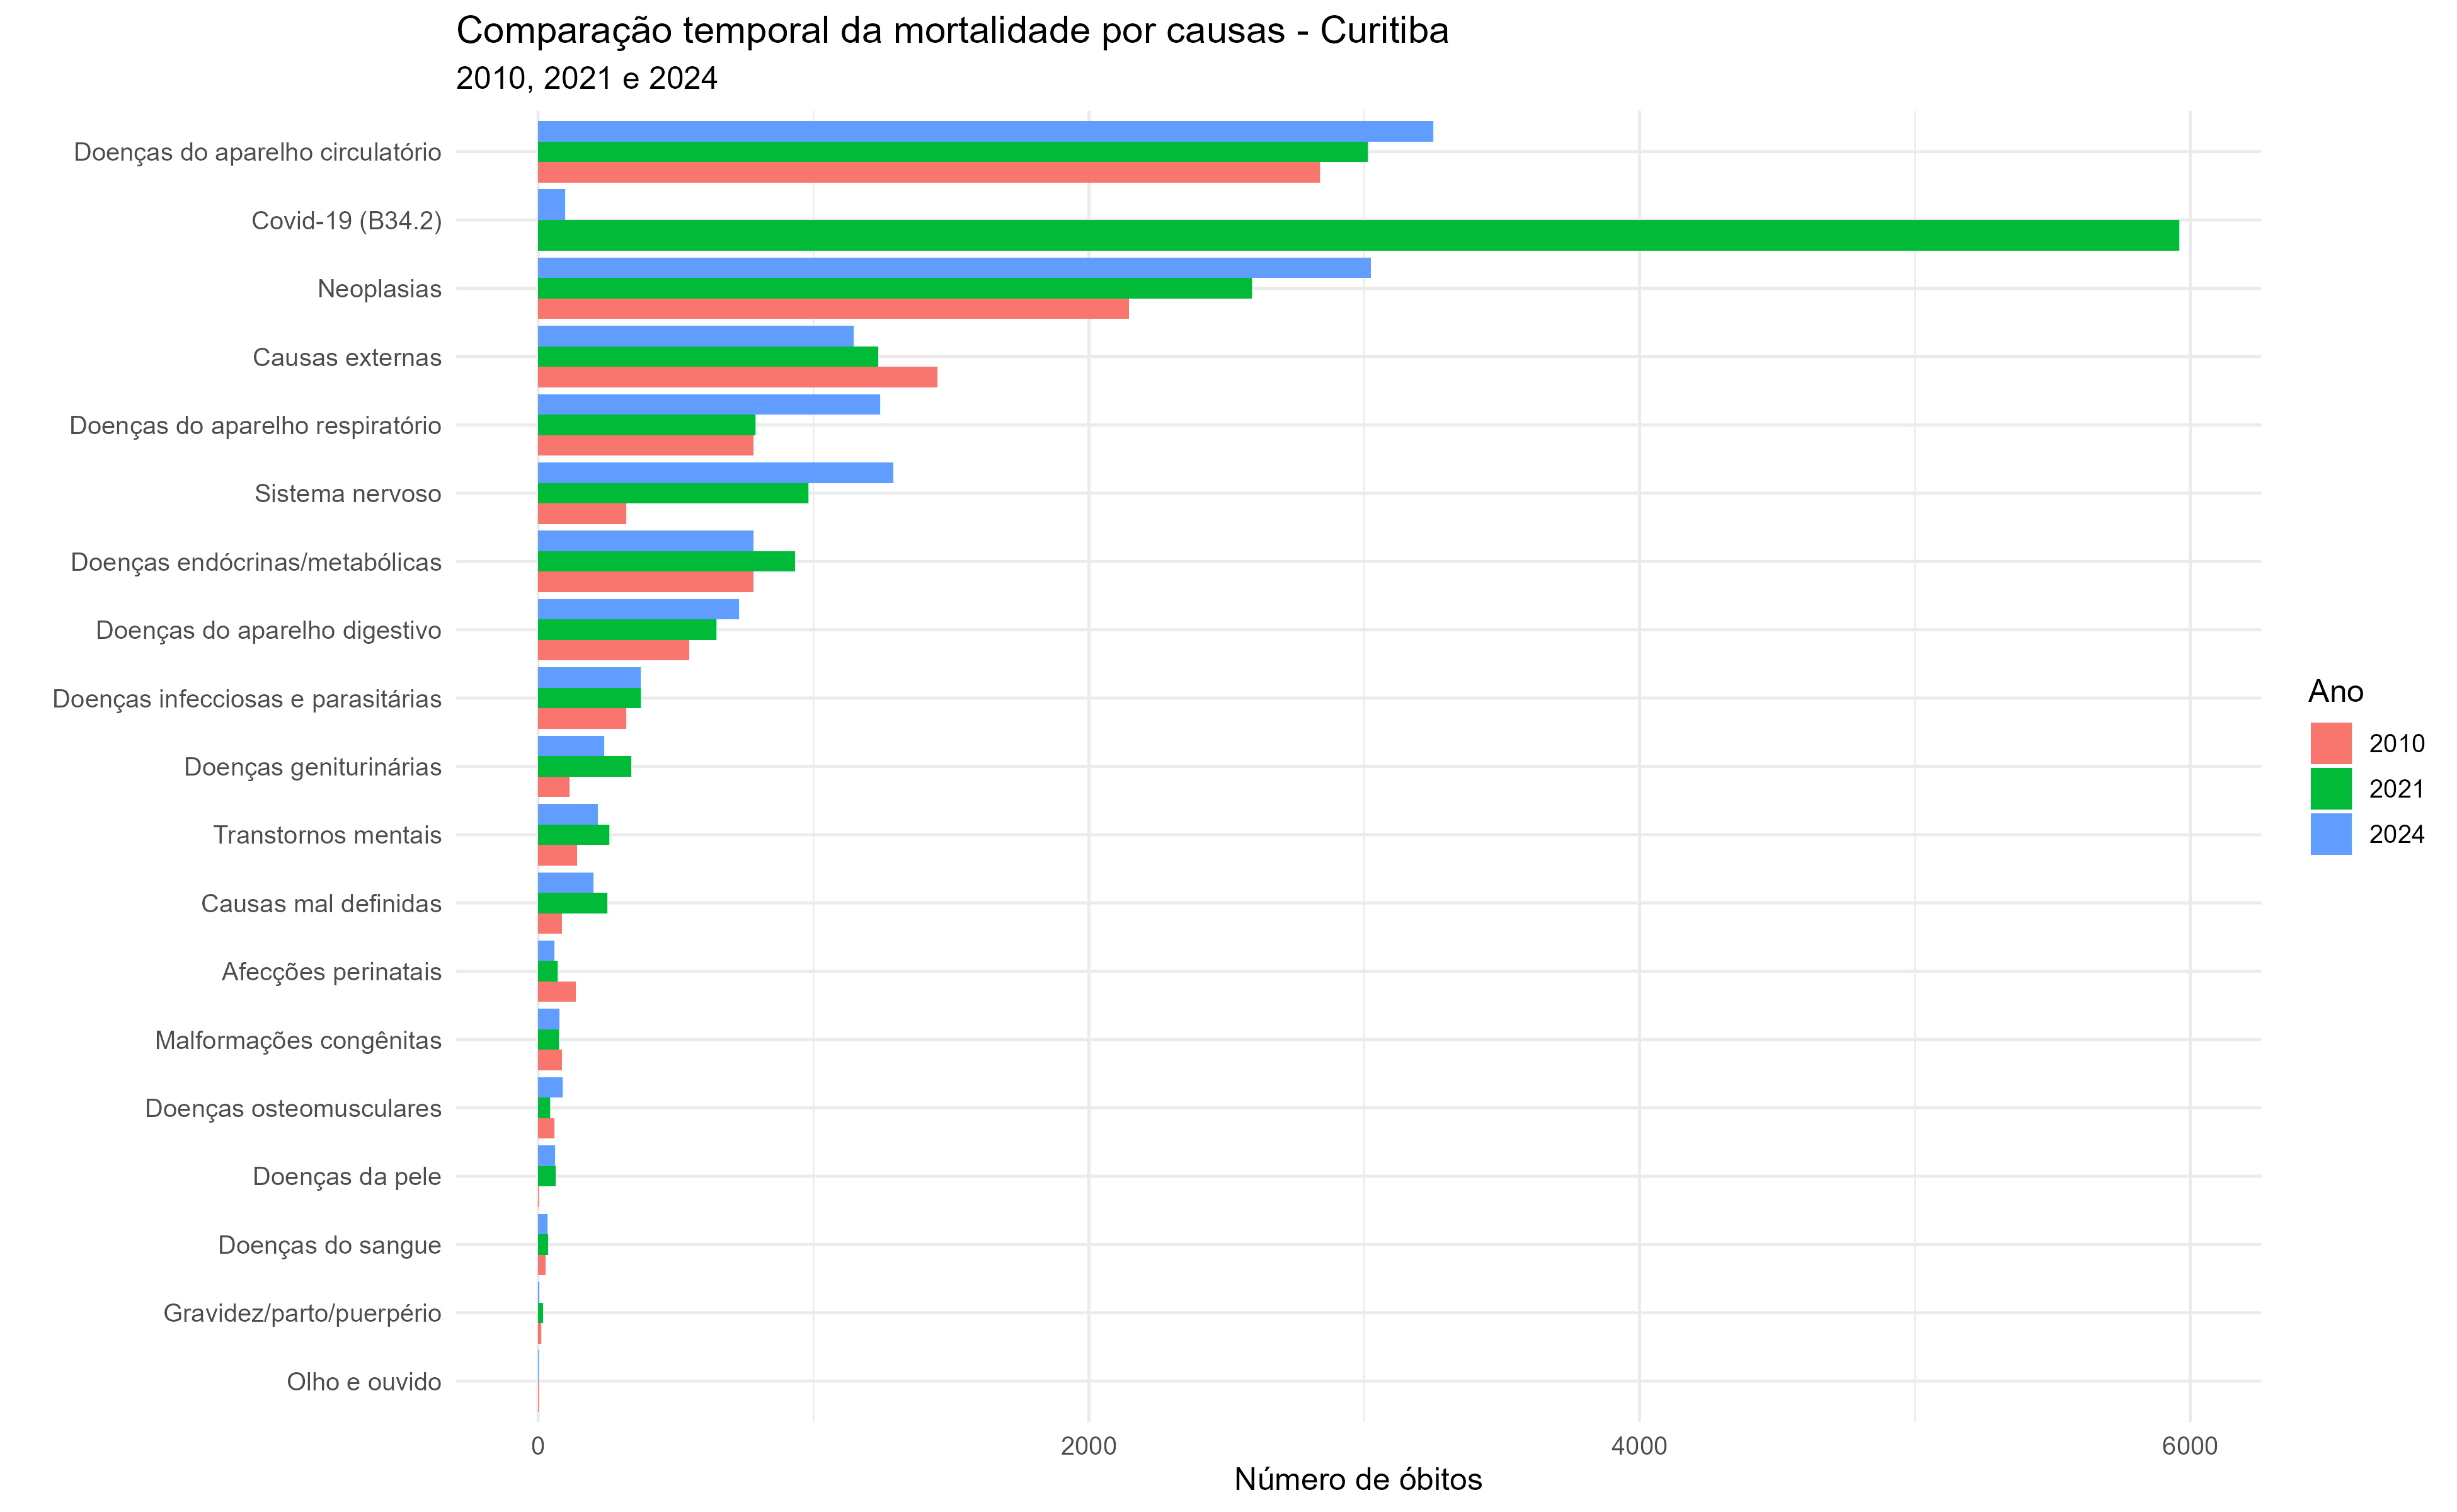
\includegraphics[width=1\linewidth,height=\textheight,keepaspectratio]{questao-3/grafico_comparacao_temporal.png}
\end{center}

\begin{center}
\pandocbounded{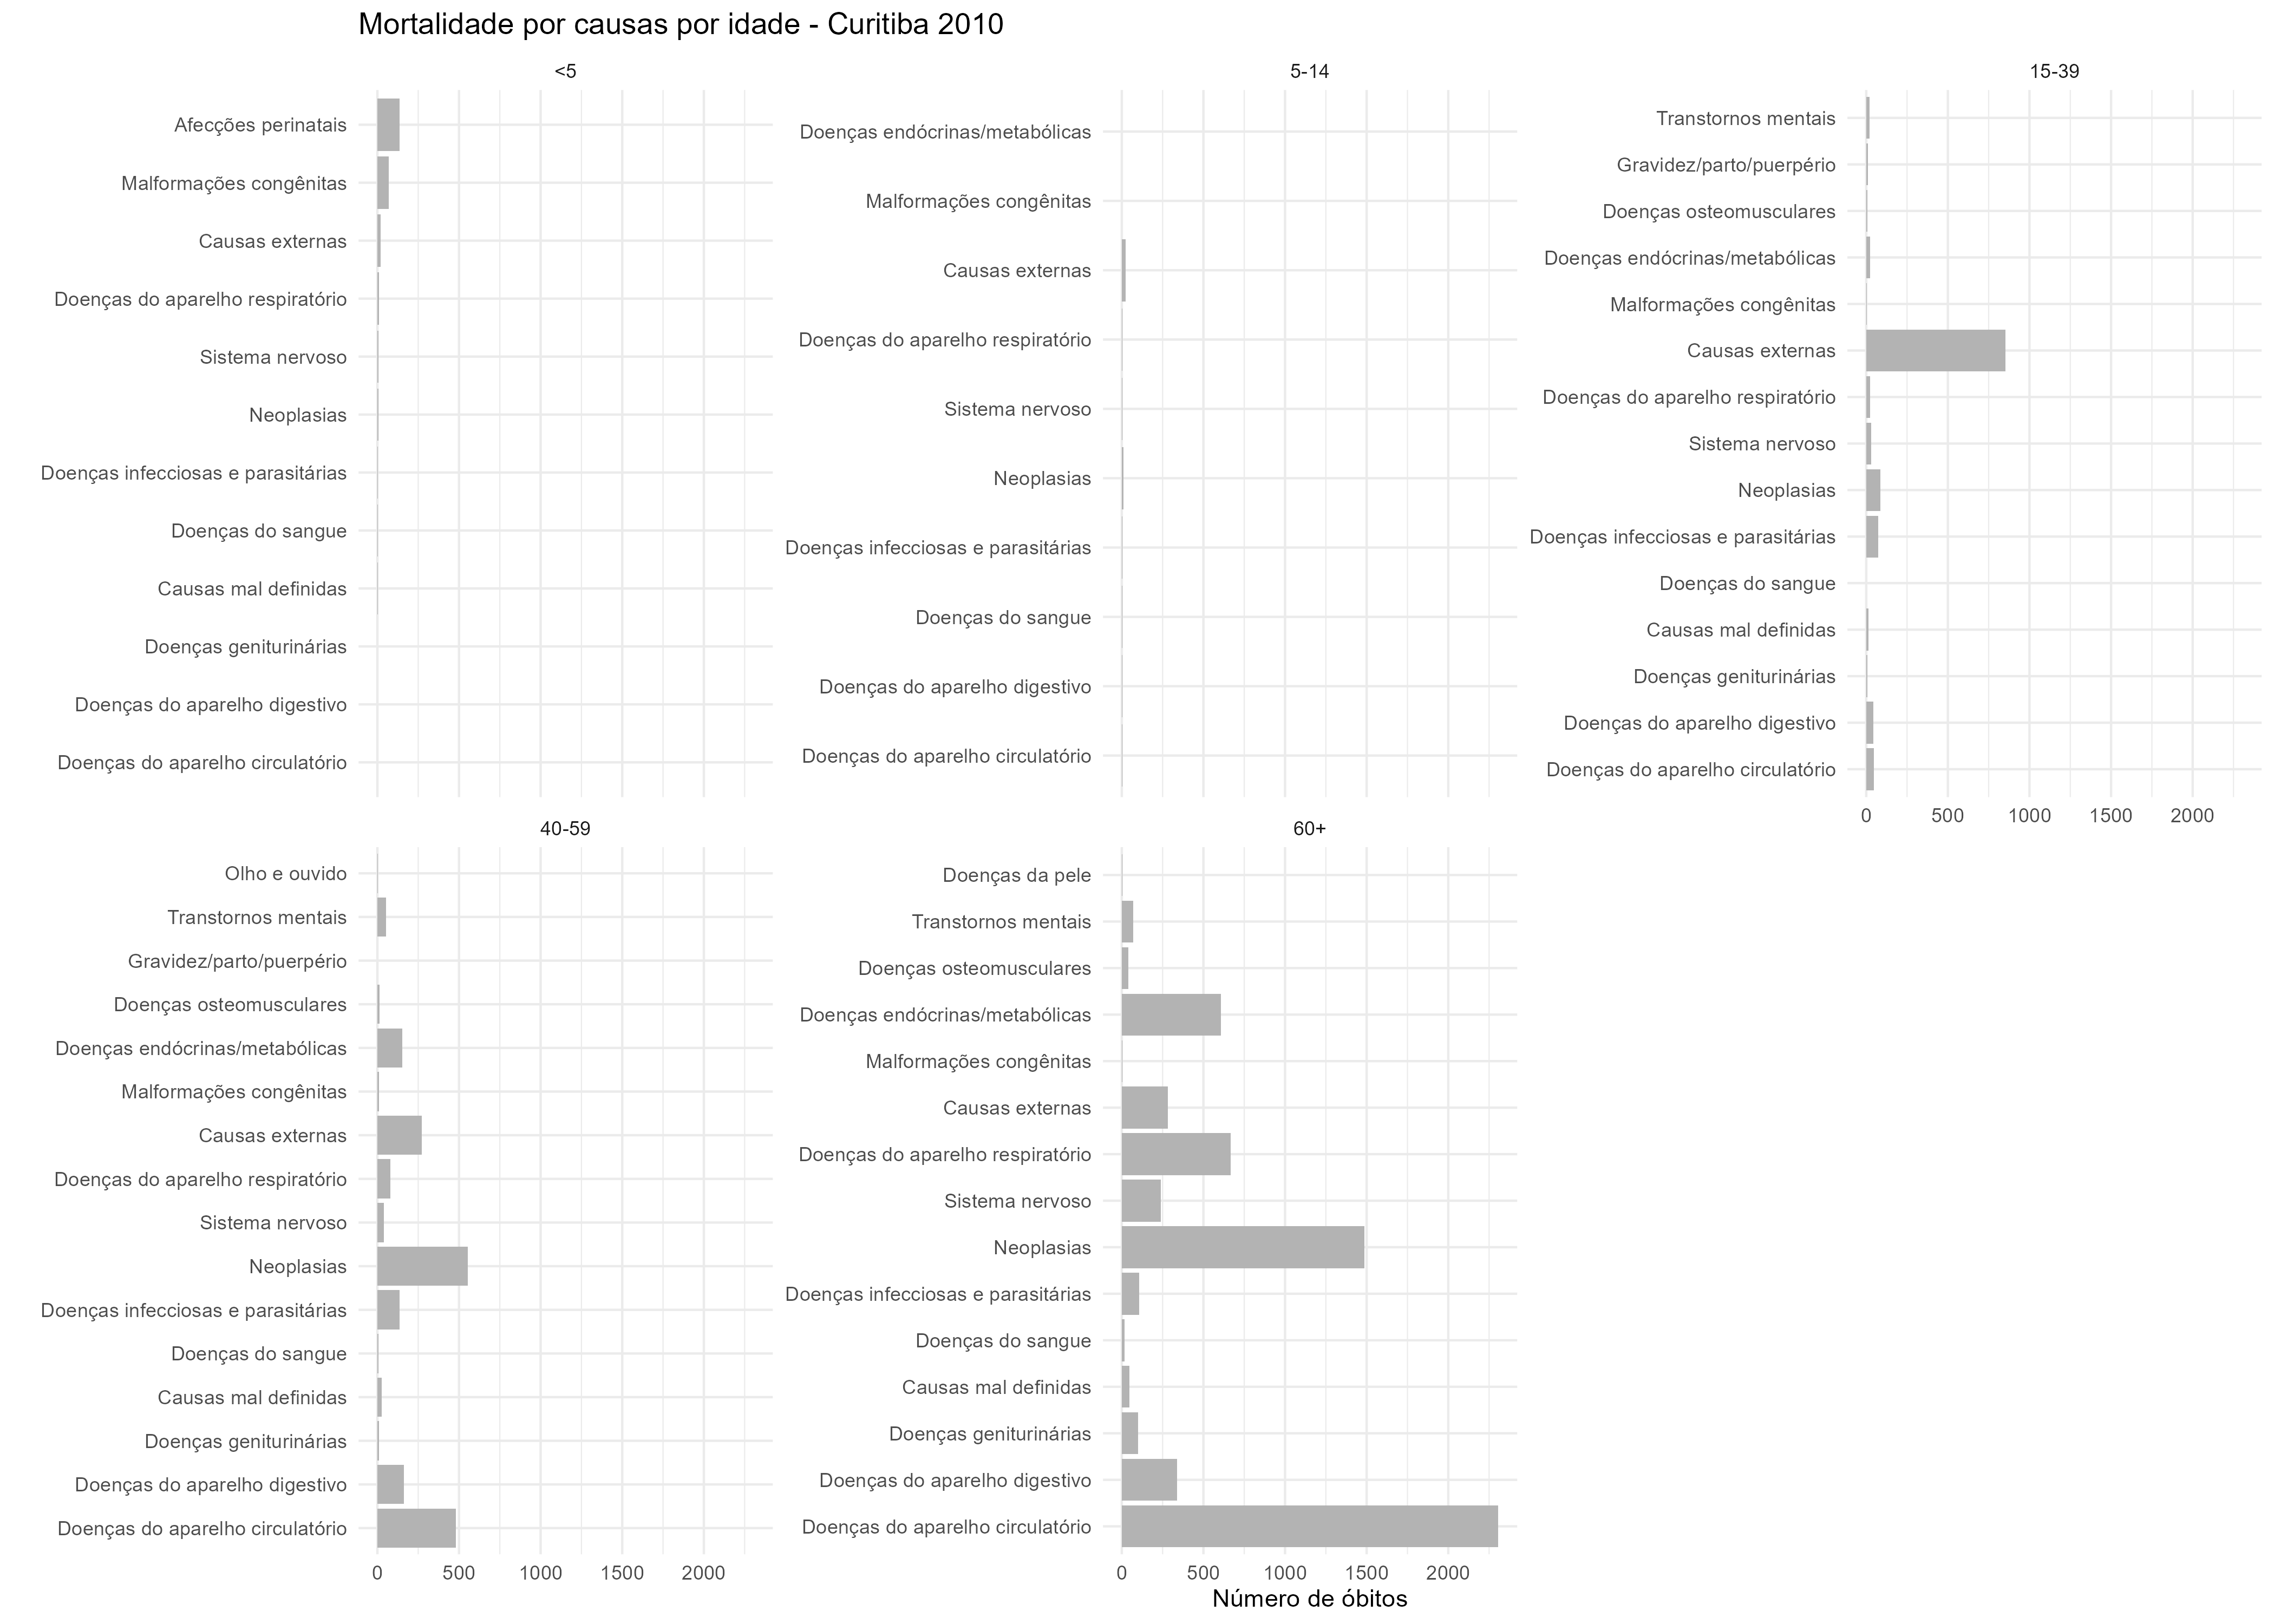
\includegraphics[keepaspectratio]{questao-3/grafico_idade_2010.png}}
\end{center}

\begin{center}
\pandocbounded{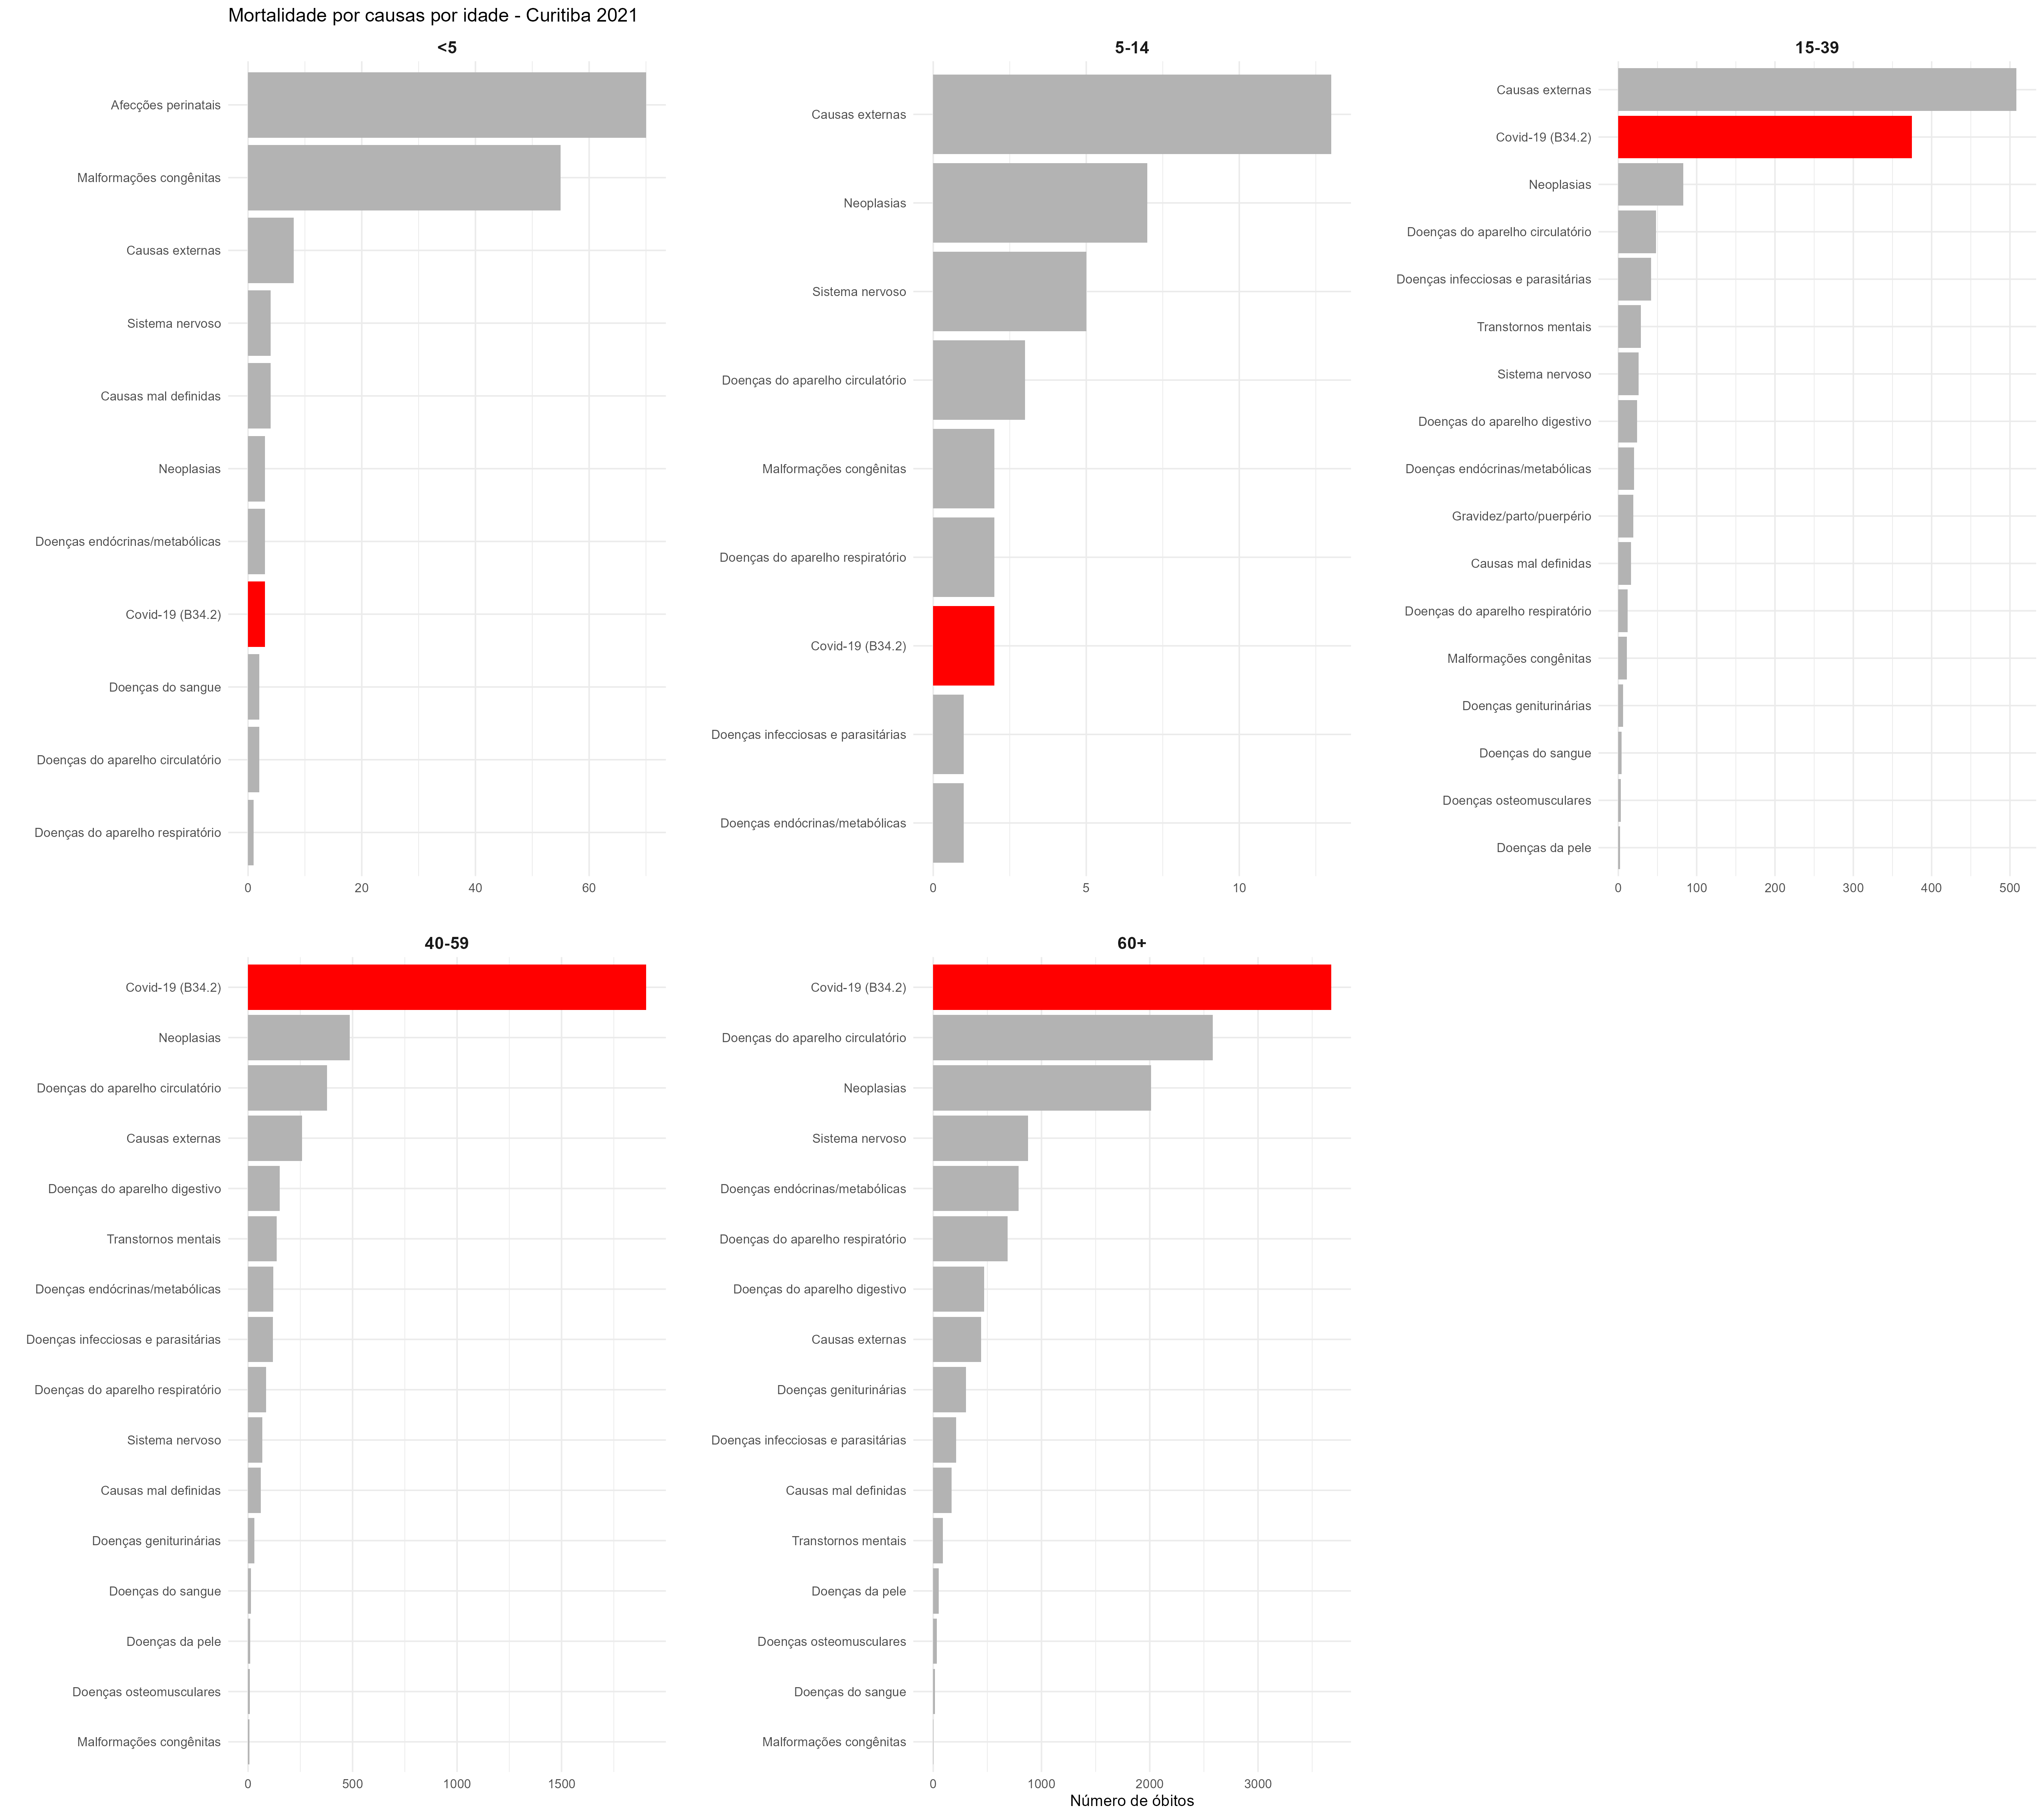
\includegraphics[keepaspectratio]{questao-3/grafico_idade_2021.png}}
\end{center}

\begin{center}
\pandocbounded{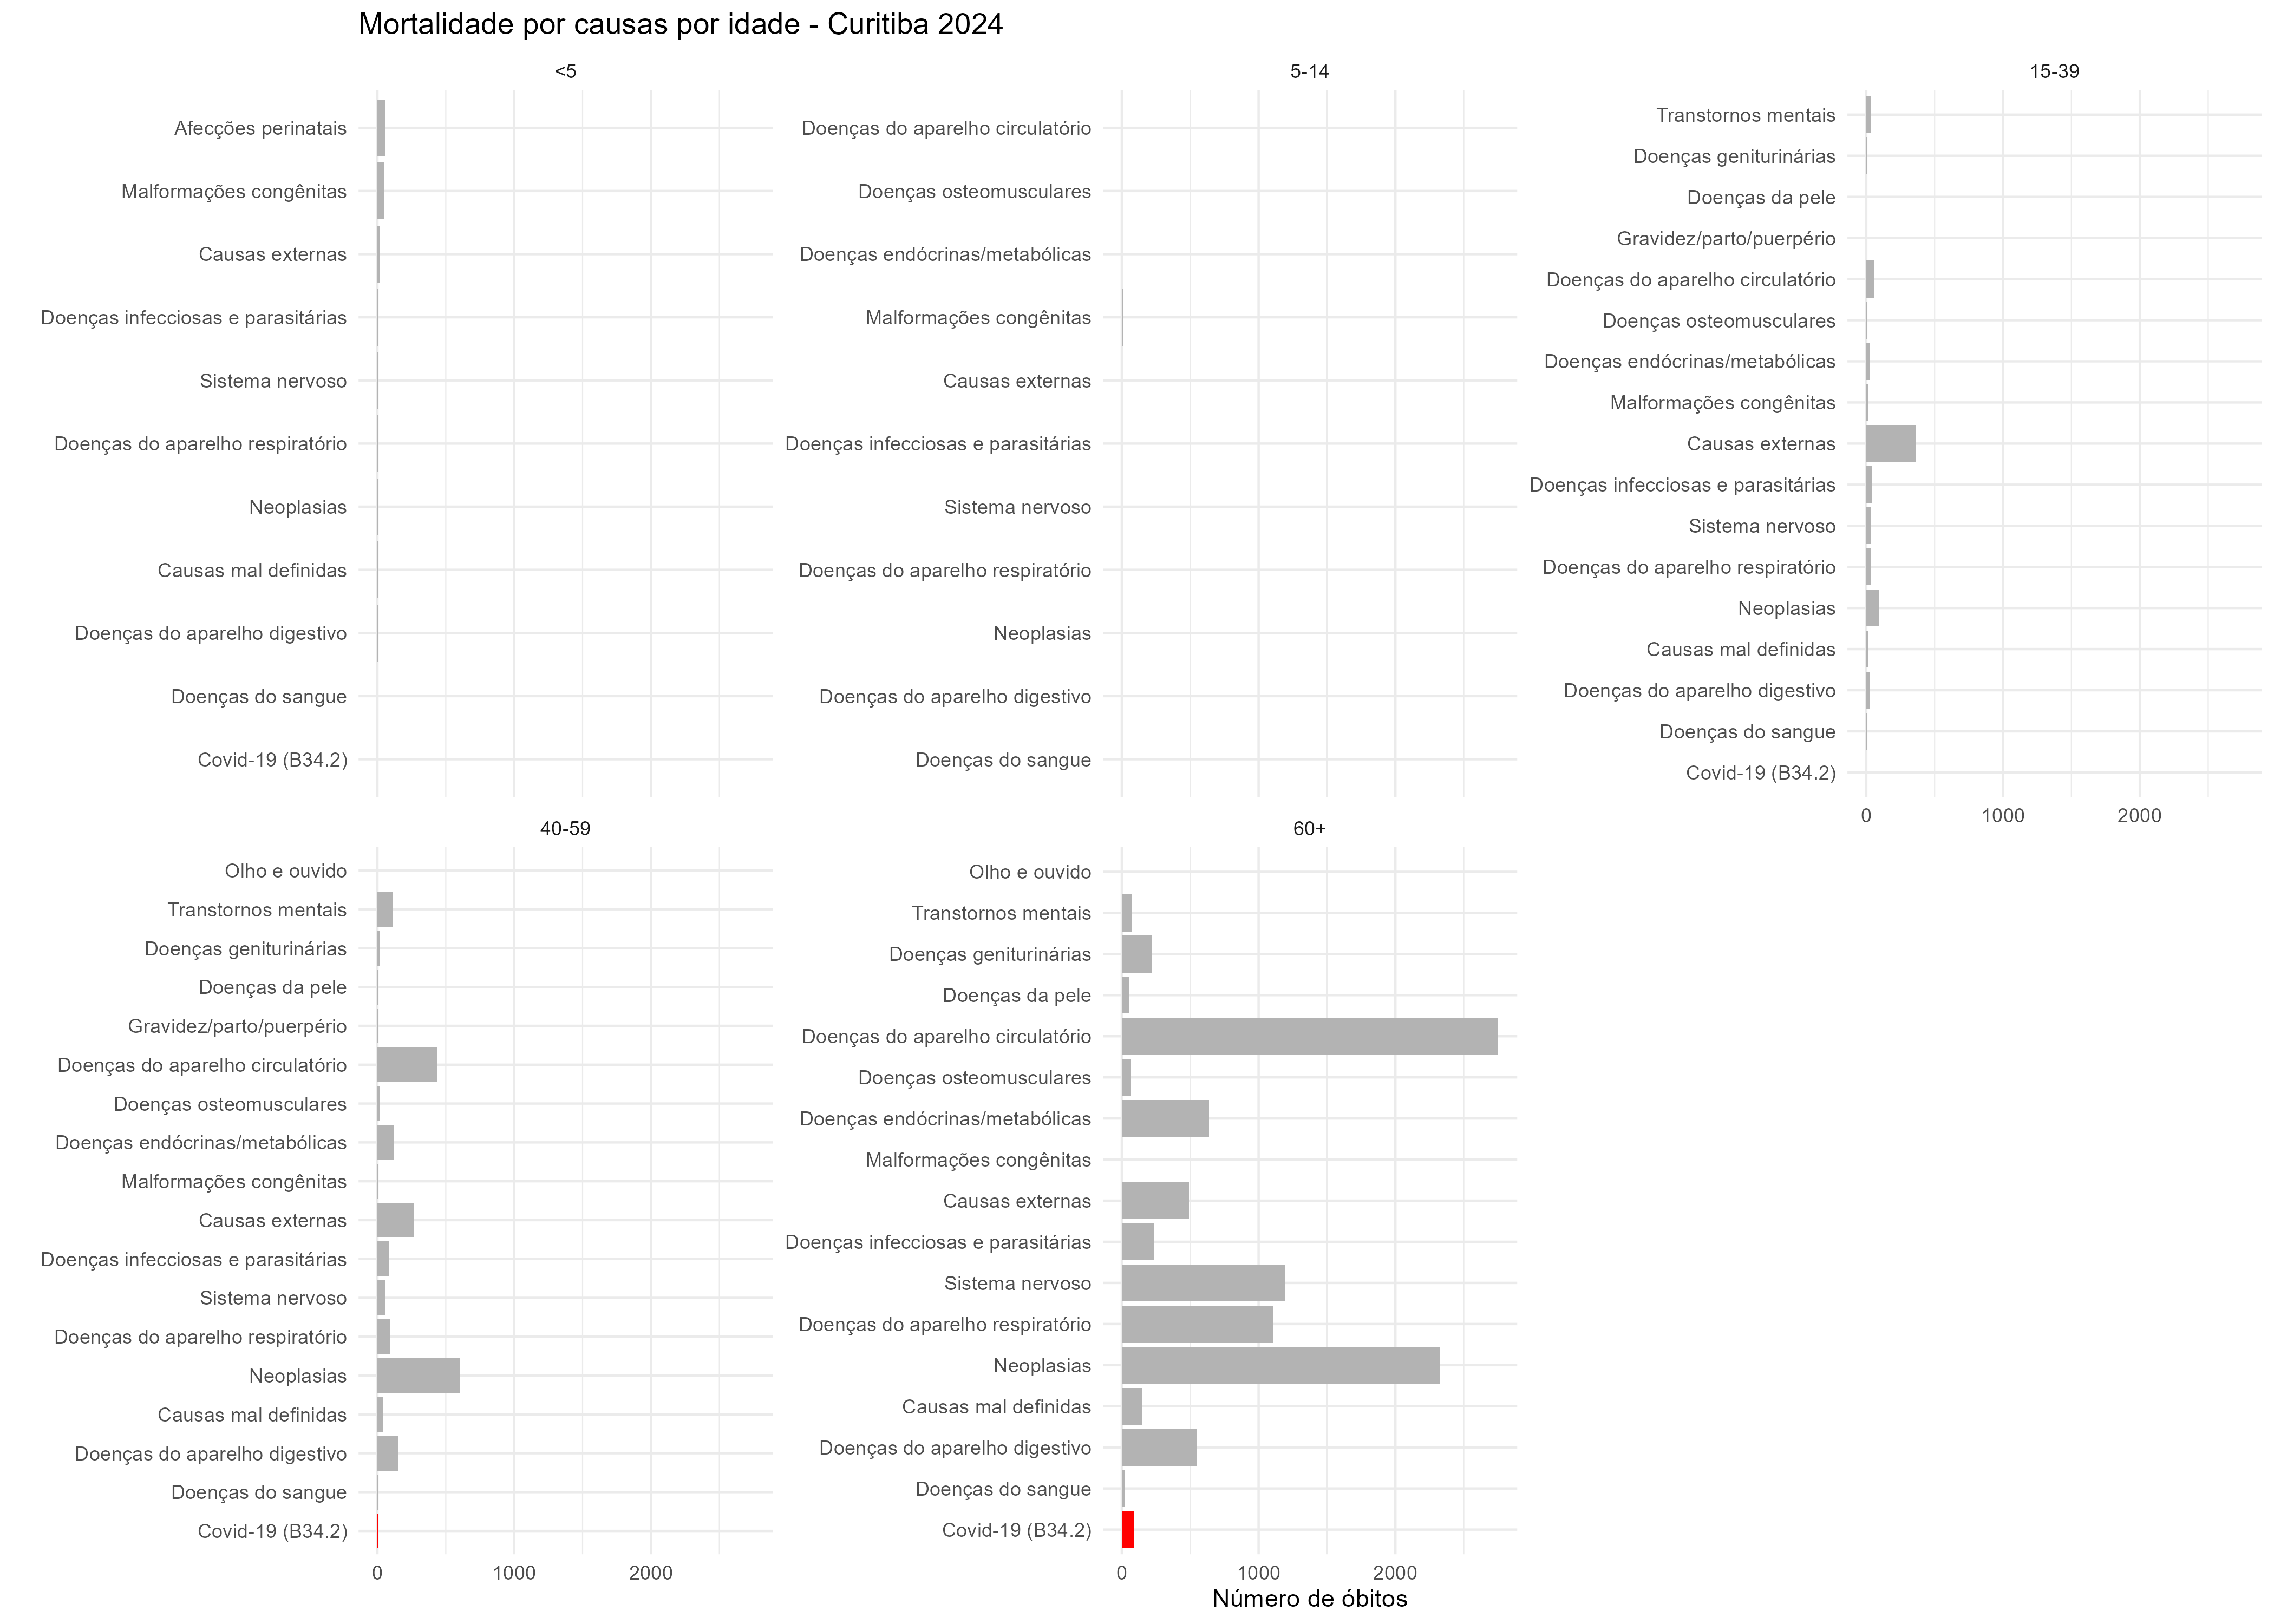
\includegraphics[keepaspectratio]{questao-3/grafico_idade_2024.png}}
\end{center}

\begin{center}
\pandocbounded{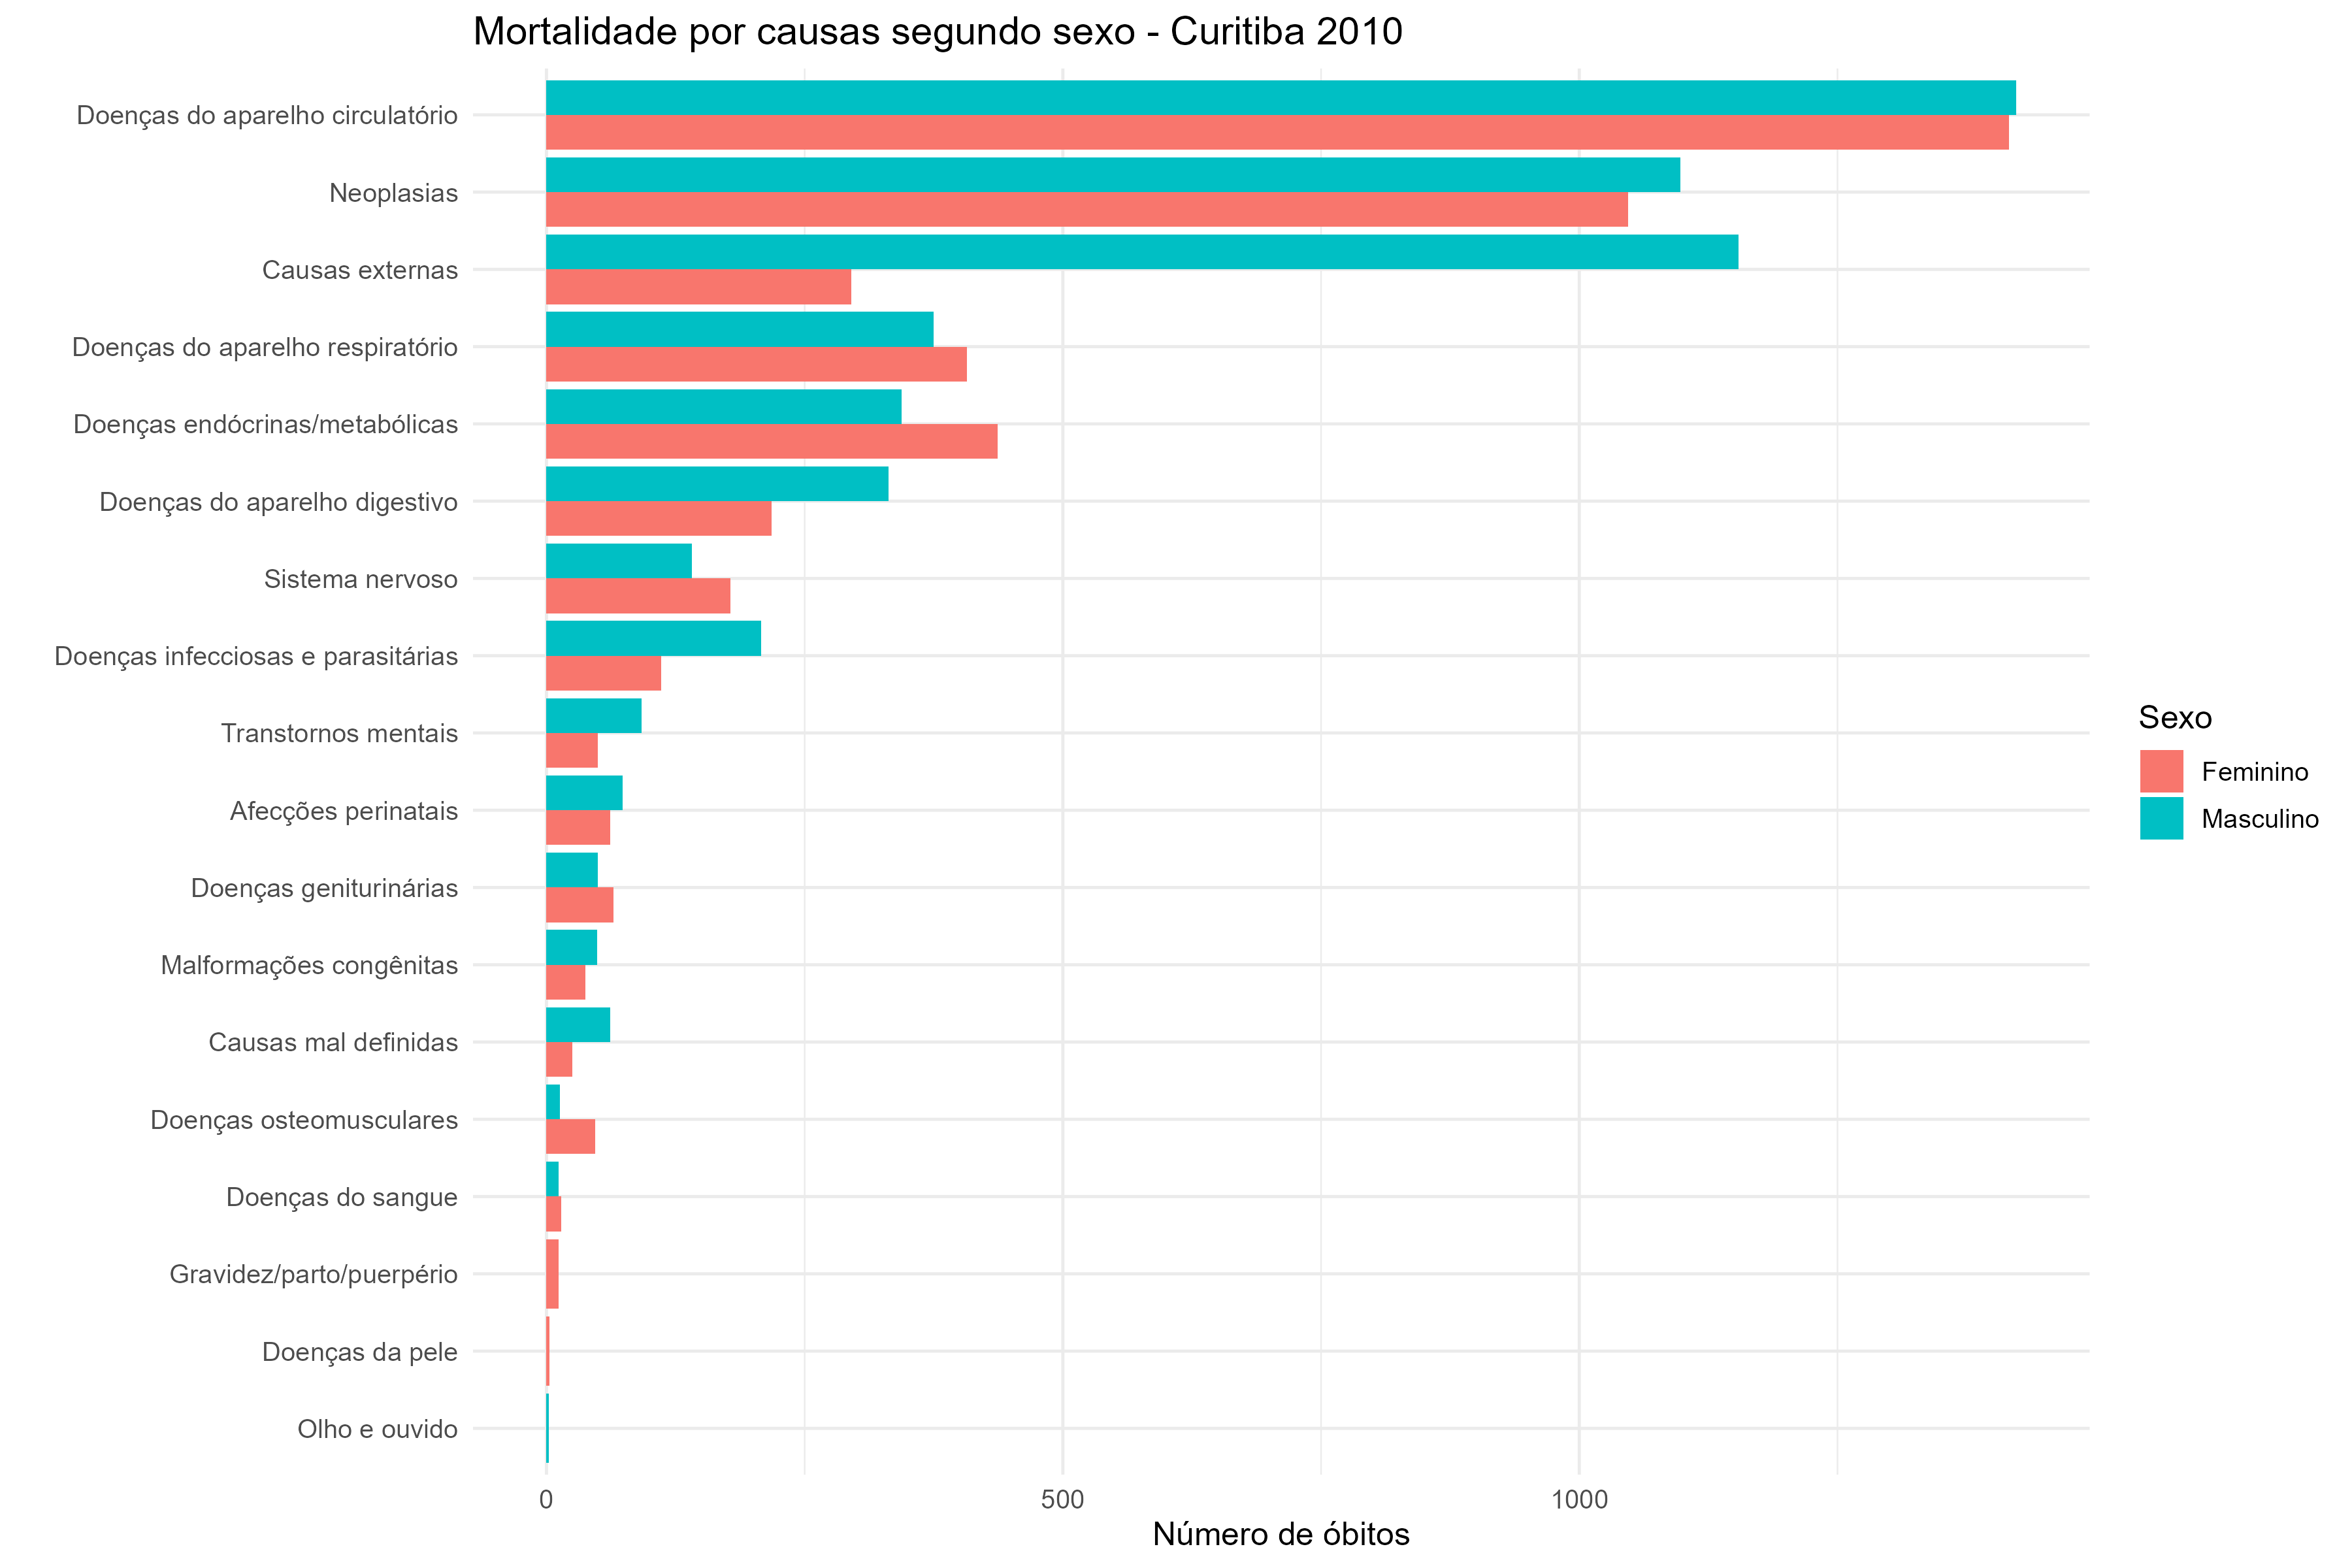
\includegraphics[keepaspectratio]{questao-3/grafico_sexo_2010.png}}
\end{center}

\begin{center}
\pandocbounded{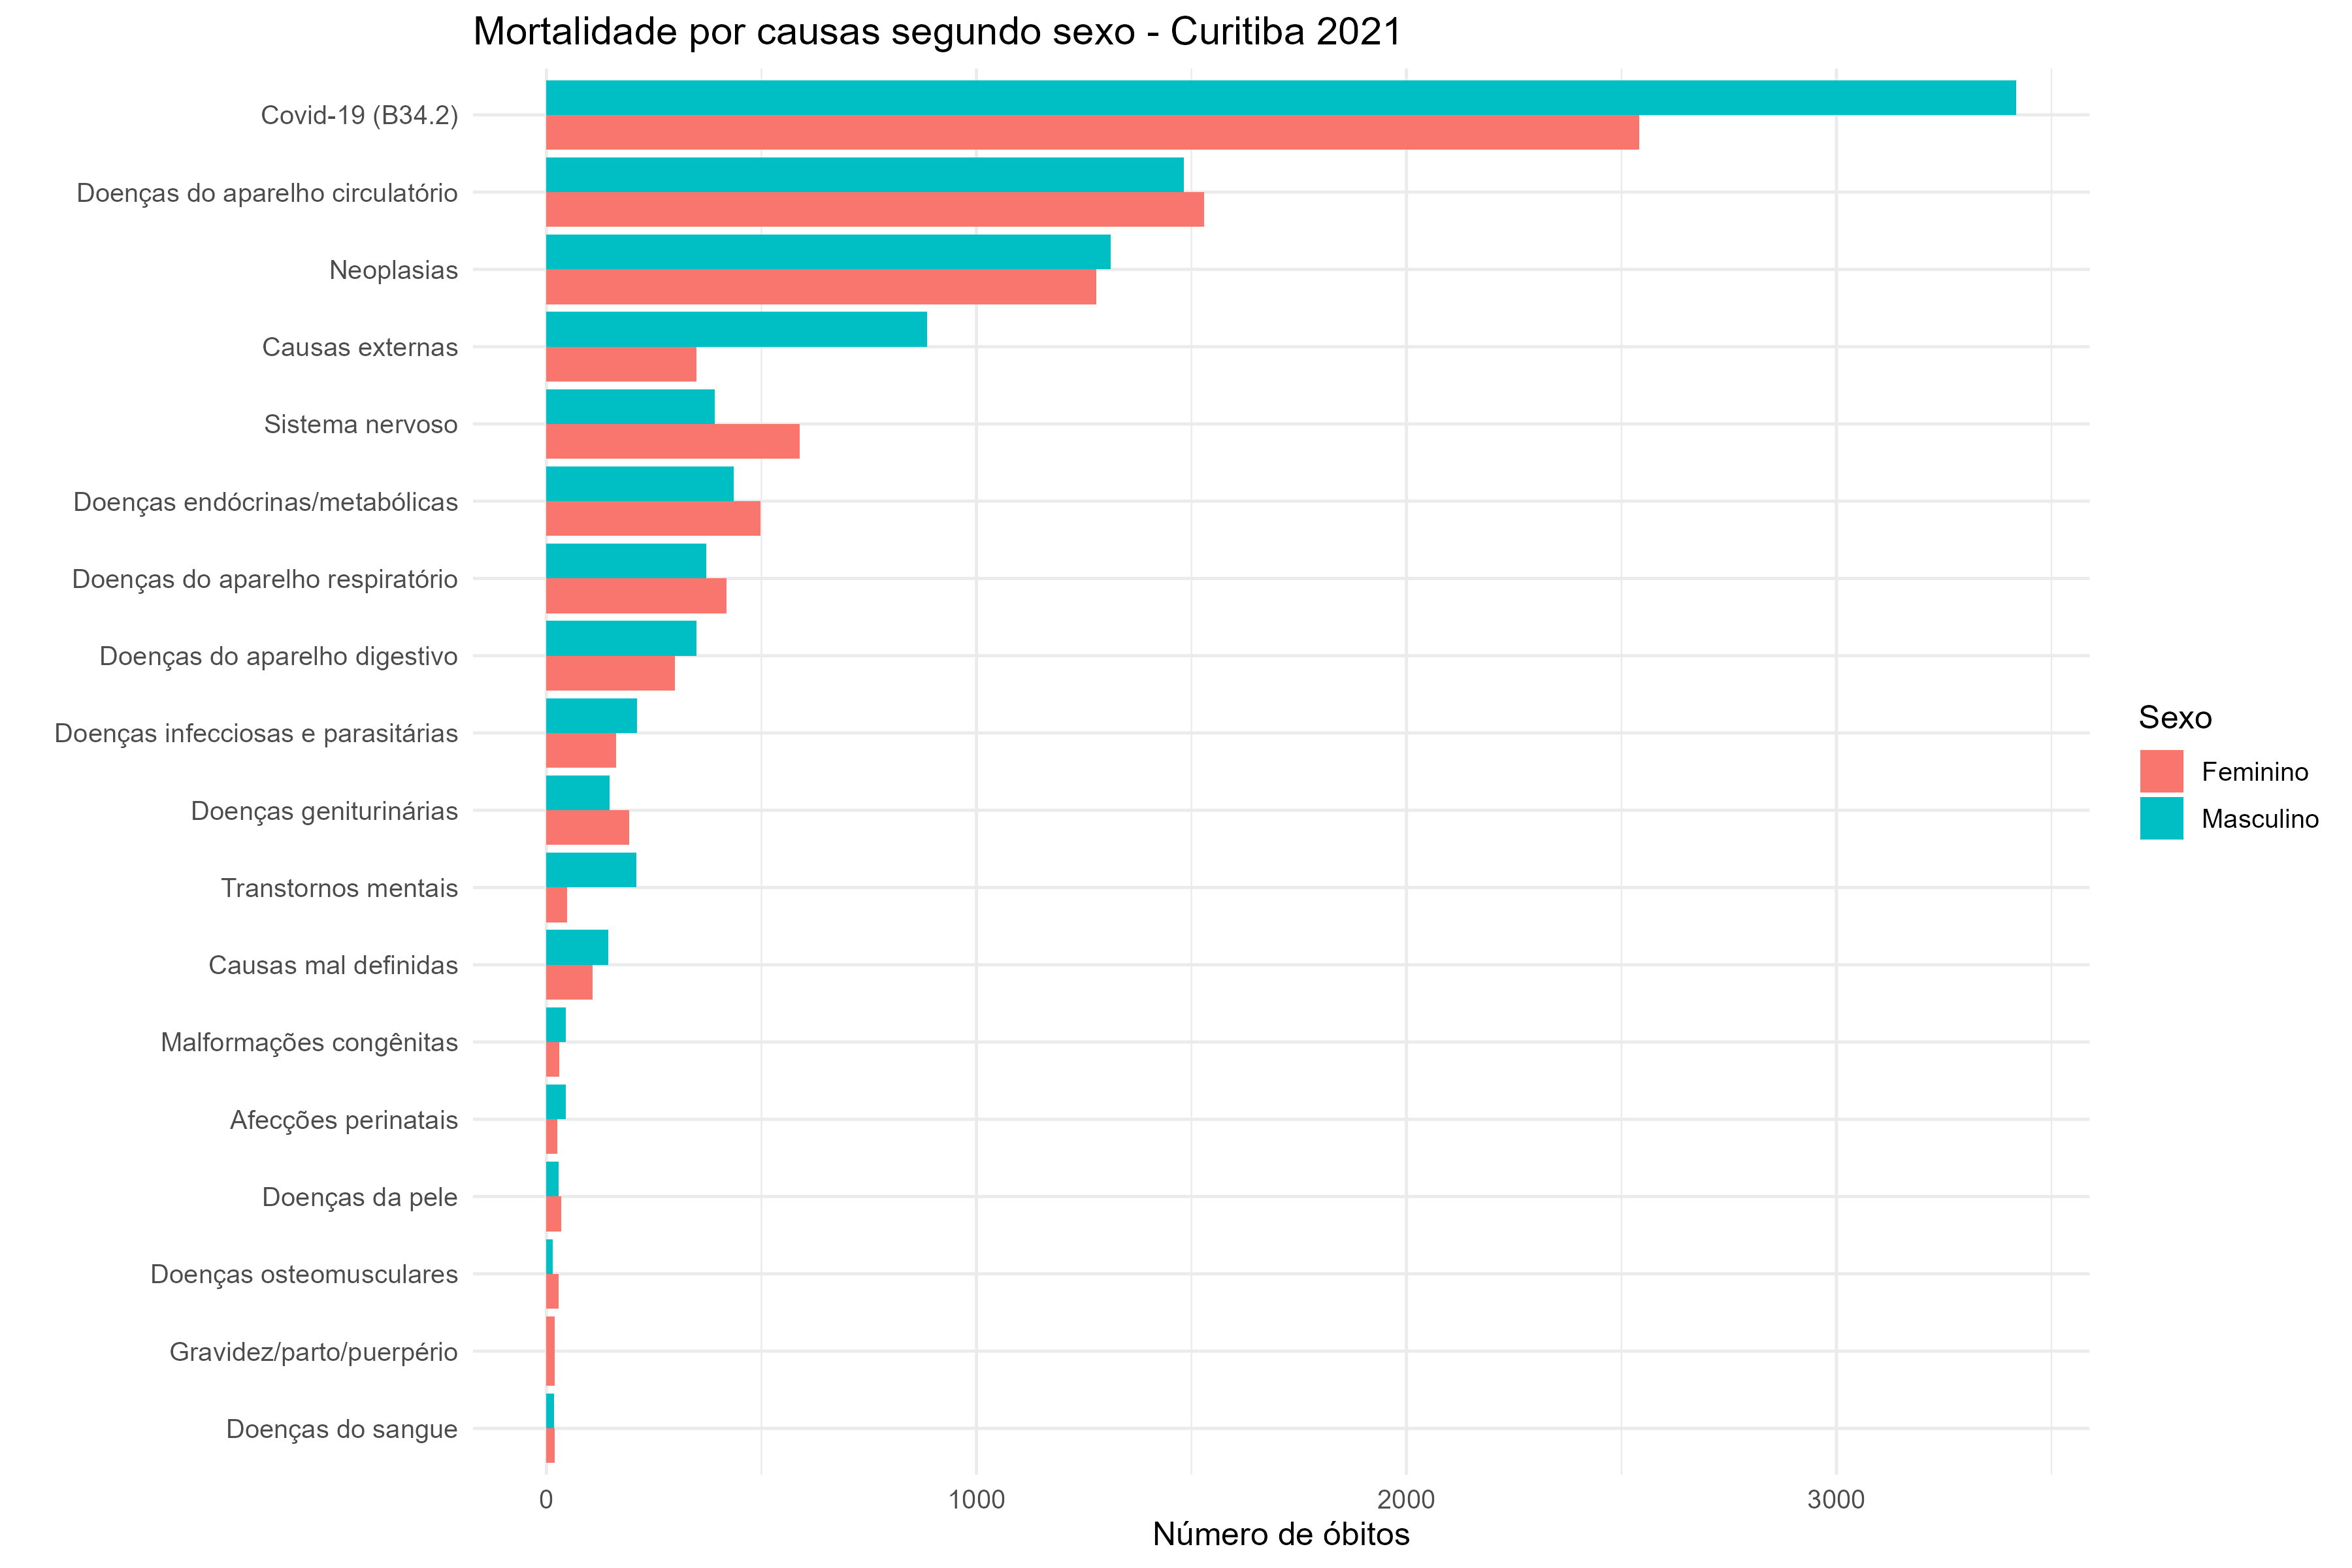
\includegraphics[keepaspectratio]{questao-3/grafico_sexo_2021.png}}
\end{center}

\begin{center}
\pandocbounded{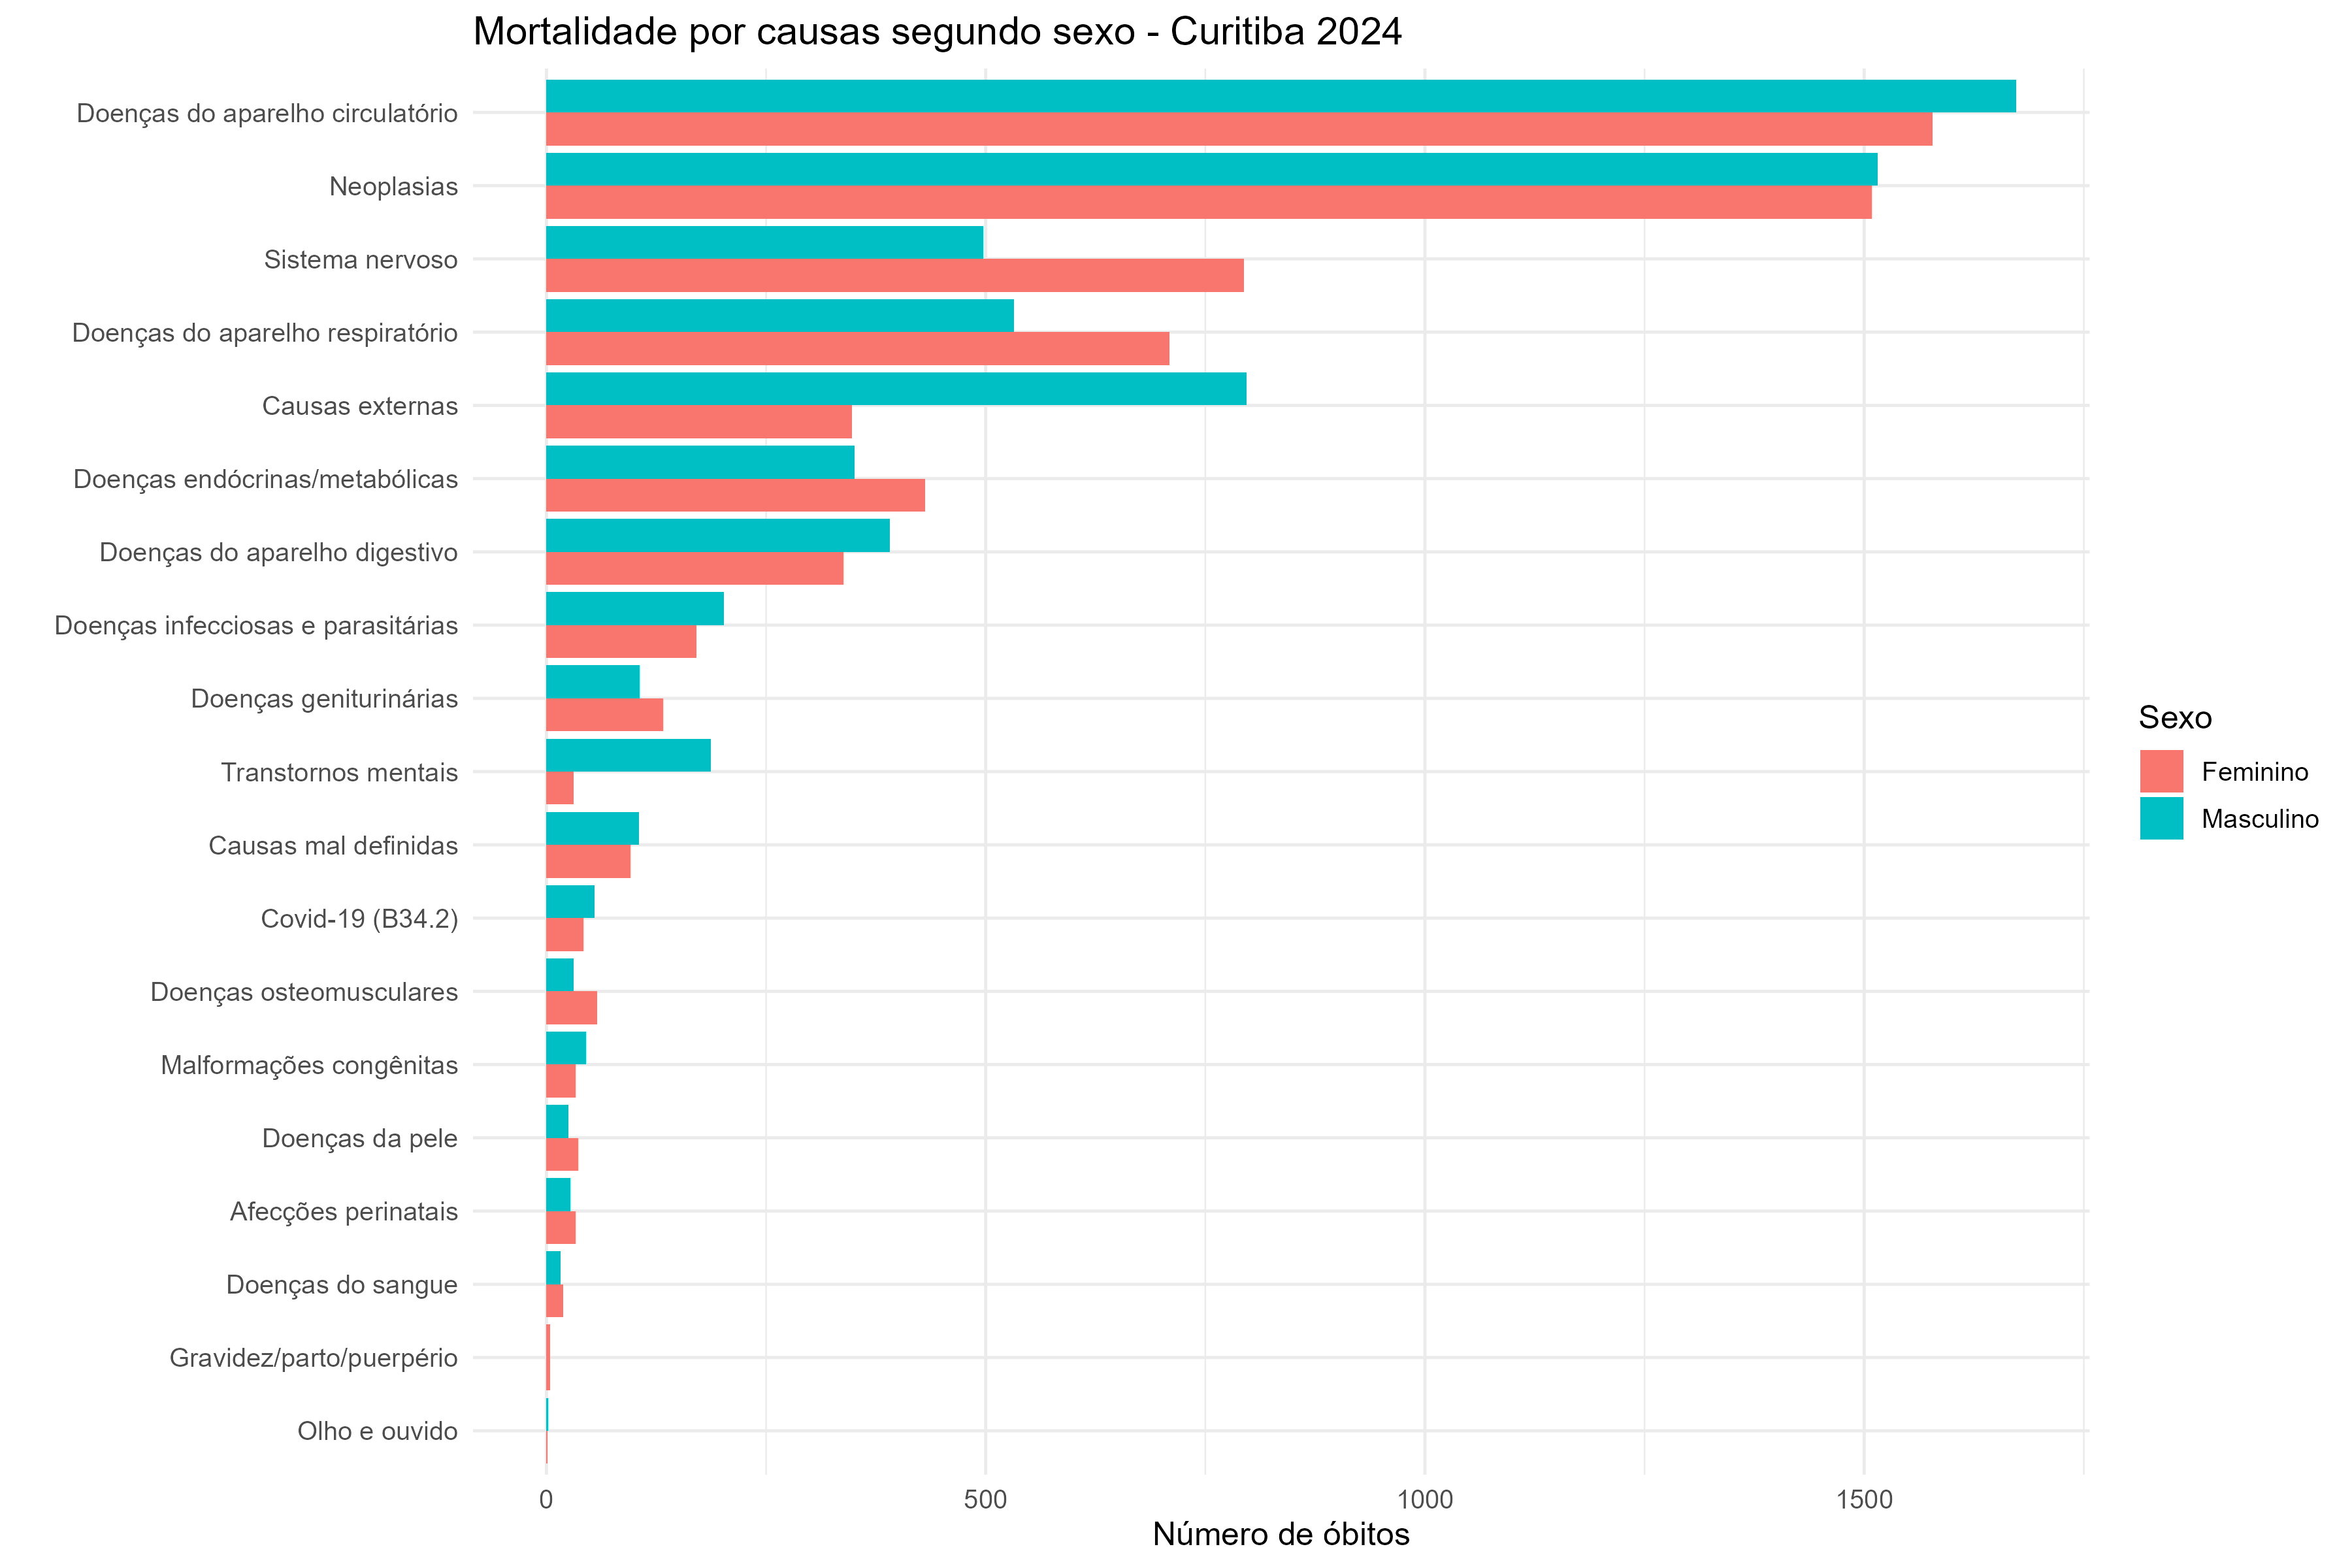
\includegraphics[keepaspectratio]{questao-3/grafico_sexo_2024.png}}
\end{center}

A estrutura de mortalidade em Curitiba apresenta, nos 3 anos observados,
um predomínio de doenças crônicas não transmissíveis, mas que sofreu um
rompimento em 2021 devido à pandemia de Covid-19. Os dados mostram que
as doenças do aparelho circulatório e as neoplasias lideram
consistentemente o volume de óbitos na população geral e na faixa de 60
anos ou mais, enquanto as causas externas --- como acidentes e violência
--- exercem um impacto maior sobre o sexo masculino e a população jovem
(15 a 39 anos). No entanto, em 2021, a Covid-19 subverteu essa
distribuição, sendo a principal causa de mortalidade em Curitiba,
registrando um volume de óbitos que praticamente duplicou em relação às
causas de morte predominantes anteriormente e afetando de forma mais
acentuada os homens em idade adulta.

Ao analisar o comportamento por subgrupos, a Covid-19 revelou impactos
diferentes a depender da idade e do sexo, poupando quase por completo os
perfis infantis, cujos óbitos permaneceram concentrados em afecções
perinatais e malformações congênitas para menores de 5 anos e em causas
externas e neoplasias para a faixa de 5 a 14 anos. Em contrapartida, a
população adulta de 40 a 59 anos e, especialmente, os idosos acima de 60
anos concentraram a maior mortalidade da pandemia em termos absolutos.
Por gênero, as disparidades se evidenciaram não apenas na maior
letalidade do vírus entre os homens, mas também na persistência da
sobremortalidade masculina por causas externas em todos os períodos
analisados.

Por fim, o cenário observado em 2024 consolida o sucesso das estratégias
de controle epidemiológico e da campanha de vacinação, demonstrando o
recuo expressivo da Covid-19 e, consequentemente, a restauração da
estrutura de mortalidade antes da pandemia. O retorno das doenças
circulatórias e das neoplasias ao topo do ranking reflete a retomada do
curso natural de transição demográfica da cidade, impulsionada pelo
envelhecimento da população que eleva o número absoluto de óbitos por
enfermidades crônicas em comparação a 2010. Assim, a comparação temporal
evidencia que, apesar do trauma epidemiológico causado pela Covid-19 em
2021, o perfil de mortalidade de Curitiba recuperou sua previsibilidade
estatística e a distribuição típica de regiões urbanas desenvolvidas.

d) Construa Tábuas de Vida para cada sexo para a UF escolhida para 2010
e 2024, a partir das taxas específicas de mortalidade obtidas no item a:

\begin{itemize}
\item
  Utilize a TMI obtida no item b. Lembre-se de que deve-se obter a TMI
  para cada sexo em separado.
\item
  Estime os fatores de separação para cada sexo, nas idades 0-1 e 1-4,
  com base nos microdados do SIM.
\item
  Compare os valores da função de esperança de vida para as idades
  exatas 0 e 60 com os obtidos no estudo do IBGE (Projeções) e no estudo
  GBD. Comente os resultados obtidos e o significado desses indicadores.
\item
  Com base na TV calculada, grafique as funções lx e nqx para cada sexo
  e comente os resultados.
\item
  Comente os resultados à luz de artigos recém publicados.
\end{itemize}

\textbf{Resposta:}

\begin{center}
\pandocbounded{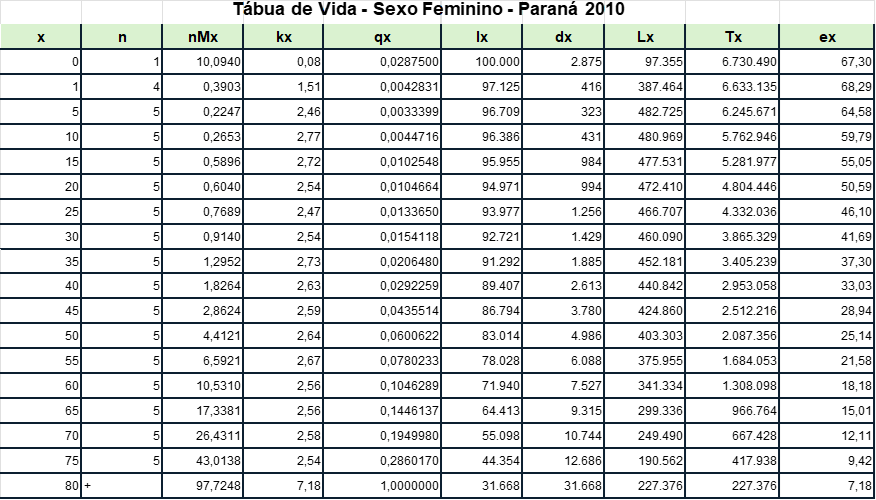
\includegraphics[keepaspectratio]{questao-3/tb_vida_fem_2010.png}}
\end{center}

\begin{center}
\pandocbounded{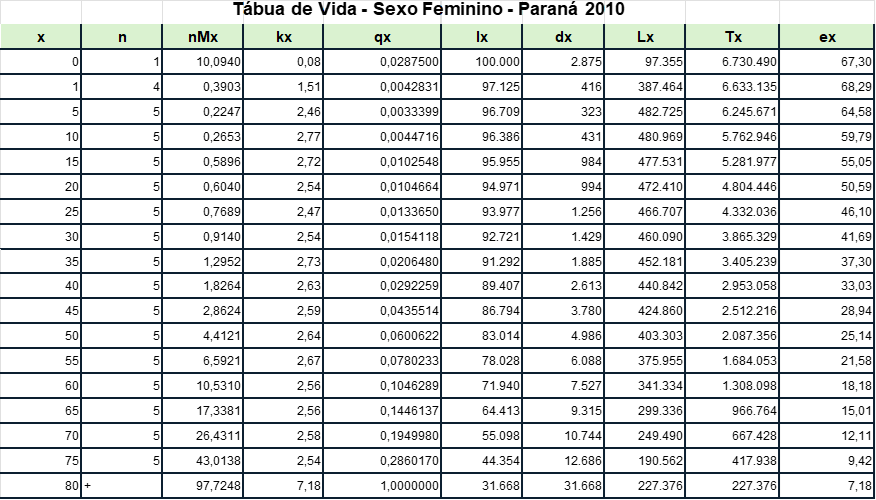
\includegraphics[keepaspectratio]{questao-3/tb_vida_fem_2010.png}}
\end{center}

\begin{center}
\pandocbounded{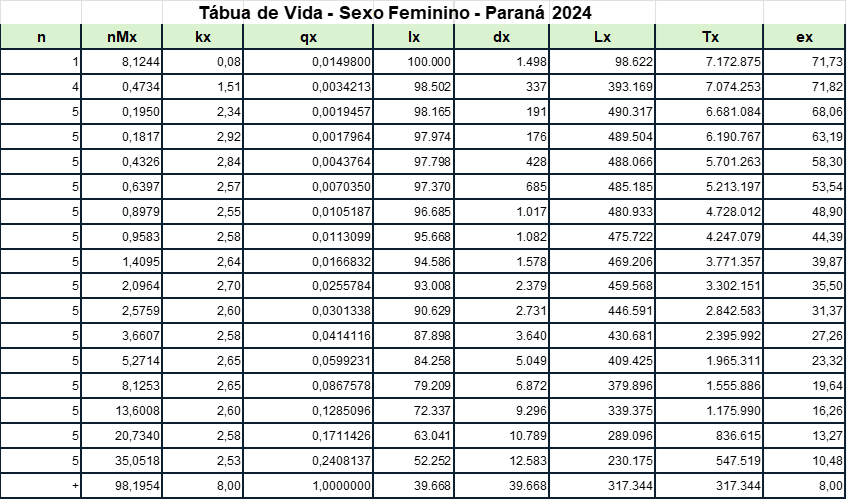
\includegraphics[keepaspectratio]{questao-3/tb_vida_fem_2024.png}}
\end{center}

\begin{center}
\pandocbounded{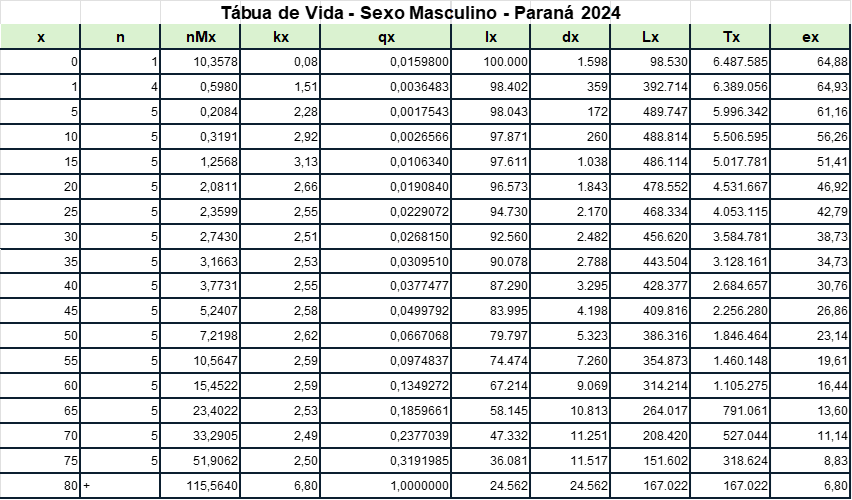
\includegraphics[keepaspectratio]{questao-3/tb_vida_masc_2024.png}}
\end{center}




\end{document}
